\documentclass[a4paper,12pt]{report}
\usepackage[utf8]{inputenc}
\usepackage{graphicx}
\usepackage{listings}
\usepackage{xcolor}
\usepackage{hyperref}
\usepackage{geometry}
\usepackage{amsmath}
\usepackage{listings}
\geometry{left=3cm, right=3cm, top=3cm, bottom=3cm}

% Code listing style
\lstset{
  numbers=left,
  numberstyle=\tiny\color{gray},
  keywordstyle=\color{blue},
  commentstyle=\color{gray},
  stringstyle=\color{red},
  breaklines=true,
  showstringspaces=false,
  basicstyle=\ttfamily\footnotesize,
  frame=single,
  language=Python
}

\begin{document}

% Cover page
\begin{titlepage}
    \centering
    \vspace*{3cm}
    {\LARGE\bfseries Program Development Report}\\[1.5cm]
    {\large Project Name: \textbf{Stappp-Q4}}\\[1cm]
    {\large Author: Lihao}\\[0.5cm]
    {\large Student ID: 2022013358}\\[0.5cm]
    {\large Institution: Xingjian College, Tsinghua University}\\[1cm]
    {\large Date: \today}
    \vfill
\end{titlepage}

% Table of contents
\tableofcontents
\newpage

% Chapters
\chapter{Introduction}
\section{Main Functions}

This program can solve finite element problems in two-dimensional or three-dimensional linear elasticity.

\subsection{element types}
The program supports the following element types:
\begin{itemize}
    \item bar element
    \item Q4 element
\end{itemize}
And it can be added to support more element types in the future.

\section{Other Functions}
The program also includes the following features:
by input file, the user can set the following parameters:
\begin{itemize}
    \item Element type
    \item Material properties
    \item Mesh generation
    \item Boundary condition setting
    \item Load application
\end{itemize}
    by output file, the user can get the following results:
\begin{itemize}
    \item Displacement field
    \item Stress field
    \item Post-processing of results
    \item Visualization of results
\end{itemize}

\chapter{Algorithm Description}
\section{Basic Procedure}
\begin{enumerate}
    \item Starting from the variational principle, use element shape functions and Gaussian quadrature to derive the element stiffness matrix and the nodal force vector corresponding to natural boundary conditions.
    
    \item Use the connectivity matrix to assemble the global stiffness matrix and the global nodal force vector.
    
    \item Apply degree of freedom (DOF) information to perform matrix reduction.
    
    \item Apply the skyline storage method to perform LU decomposition of the stiffness matrix and solve for the nodal displacements.
    
    \item Use the nodal displacements to compute stresses at superconvergent stress points and perform visualization and analysis.
\end{enumerate}

\[
\delta \Pi = \delta \int_{\Omega} \left( \frac{1}{2} \varepsilon^T \mathbf{D} \varepsilon - \mathbf{u}^T \mathbf{f} \right) d\Omega - \delta \int_{\Gamma_t} \mathbf{u}^T \bar{\mathbf{t}} \, d\Gamma = 0
\]

\[
\mathbf{K}^e = \int_{\Omega^e} \mathbf{B}^T \mathbf{D} \mathbf{B} \, d\Omega, \quad 
\mathbf{f}^e = \int_{\Omega^e} \mathbf{N}^T \mathbf{f} \, d\Omega + \int_{\Gamma_t^e} \mathbf{N}^T \bar{\mathbf{t}} \, d\Gamma
\]

\[
\mathbf{K} = \sum_e \mathbf{B}_e^T \mathbf{K}^e \mathbf{B}_e, \quad 
\mathbf{f} = \sum_e \mathbf{B}_e^T \mathbf{f}^e
\]

\[
\begin{bmatrix}
\mathbf{K}_{II} & \mathbf{K}_{IB} \\
\mathbf{K}_{BI} & \mathbf{K}_{BB}
\end{bmatrix}
\begin{bmatrix}
\mathbf{u}_I \\
\mathbf{u}_B
\end{bmatrix}
=
\begin{bmatrix}
\mathbf{f}_I \\
\mathbf{f}_B
\end{bmatrix}
\]

\[
\Rightarrow \quad
\mathbf{K}_{II} \mathbf{u}_I = \mathbf{f}_I - \mathbf{K}_{IB} \bar{\mathbf{u}}
\]

\[
\mathbf{K}_r = \mathbf{L} \mathbf{U}, \quad 
\mathbf{L} \mathbf{y} = \mathbf{f}_r, \quad 
\mathbf{U} \mathbf{u}_r = \mathbf{y}
\]

\[
\sigma = \mathbf{D} \mathbf{B} \mathbf{u}
\]

\chapter{Instructions for Use}
\section{Input File Format}

The input file should be structured as follows:
The input file consists of the following sections:

\paragraph{Header Line}  
A brief description of the problem to be solved.

\paragraph{Control Line}  
Enter the following parameters (separated by spaces or commas):
\begin{itemize}
  \item \texttt{NUMNP}: Total number of nodes
  \item \texttt{NUMEG}: Total number of element groups (each group contains elements of the same type)
  \item \texttt{NLGASE}: Number of load cases
  \item \texttt{MODEX}: Solution mode (0 = data check only, 1 = perform solution)
  \item \texttt{DIM}: Dimension of the problem (2 or 3)
\end{itemize}

\paragraph{Node Data}  
List node information in order from 1 to \texttt{NUMNP}. Each line includes:
\begin{itemize}
  \item Node number
  \item Boundary condition codes in the $x$, $y$, and $z$ directions (0 = free, 1 = fixed)
  \item Coordinates in the $x$, $y$, and $z$ directions
\end{itemize}

\paragraph{Load Data (total of \texttt{NLGASE} cases)}  
Each load case includes:
\begin{itemize}
  \item \textbf{Load Control Line}:
    \begin{itemize}
      \item Load case number
      \item Number of concentrated loads
    \end{itemize}
  \item \textbf{Load Data Lines}:
    \begin{itemize}
      \item Node number
      \item Load direction (1 = $x$, 2 = $y$, 3 = $z$)
      \item Load value
    \end{itemize}
\end{itemize}

\paragraph{Element Group Data (total of \texttt{NUMEG} groups)}  
Each group contains:
\begin{itemize}
  \item \textbf{Element Group Control Line}:
    \begin{itemize}
      \item Element type (e.g., 1 = truss/bar, 2 = Q4 element)
      \item Number of elements (\texttt{NUME})
      \item Number of material property sets (\texttt{NUMMAT})
      \item Integration scheme (0 = full, 1 = reduced)
    \end{itemize}
  \item \textbf{Material Property Data} (\texttt{NUMMAT} lines):
    \begin{itemize}
      \item Property set number
      \item Young's modulus
      \item Cross-sectional area (for bar elements)
      \item Poisson's ratio and thickness (for plane elements)
    \end{itemize}
  \item \textbf{Element Data} (\texttt{NUME} lines):
    \begin{itemize}
      \item Element number
      \item Left and right node numbers
      \item Property set number
    \end{itemize}
\end{itemize}
\begin{lstlisting}[basicstyle=\ttfamily, frame=single, caption={test1\_2.dat}]
Cables to test STAP++
6    1  1  1  2
1    1  1  0  0
2    0  0  1  0
3    0  0  2  0
4    1  1  0  1
5    0  0  1  1
6    0  0  2  1
1    2
6    1  1
3    1  -1
2    2  1  0
1    100  0.3  1
1    1  2  5  4  1
2    2  3  6  5  1
\end{lstlisting}
\subsection{Visualization of results}
Run \texttt{postprocessing.py}, input the output filename generated by \texttt{stap++.exe}, and enter the deformation magnification factor. The program will plot the structure before and after deformation.

\chapter{Verification of Computational Accuracy}
\section{patch test}
The patch test is a fundamental verification method for finite element codes. It ensures that the code can accurately solve simple problems, such as a uniform stress field in a square or cube, without introducing numerical errors.
\subsection{input file}
\begin{lstlisting}[basicstyle=\ttfamily, frame=single, caption={patch\_test.dat}]
 Cables to test STAP++
8     1     1     1     2
1     1     1     0     0
2     0     1     1     0
3     0     0     1     1
4     0     0     0     1
5     0     0     0.25  0.25
6     0     0     0.75  0.25
7     0     0     0.75  0.75
8     0     0     0.25  0.75
1     2
3     2    -1
4     2    -1
2     5     1     0
1   100   0.3     1
1     1     2     6     5     1
2     6     2     3     7     1
3     8     7     3     4     1
4     1     5     8     4     1
5     5     6     7     8     1
\end{lstlisting} 
\subsection{output file}
\begin{lstlisting}[basicstyle=\ttfamily\scriptsize, frame=single, caption={patch\_test.out}]
TITLE : Cables to test STAP++ (15:38:24 on June 4, 2025, Wednesday)

CONTROL INFORMATION
NUMBER OF NODAL POINTS...........(NUMNP) = 8
NUMBER OF ELEMENT GROUPS.........(NUMEG) = 1
NUMBER OF LOAD CASES.............(NLCASE)= 1
SOLUTION MODE....................(MODEX) = 1
  EQ.0, DATA CHECK
  EQ.1, EXECUTION

NODAL POINT DATA
NODE   BOUNDARY              NODAL POINT
NUM    CONDITION             COORDINATES
1      1 1                   0.00000e+00 0.00000e+00
2      0 1                   1.00000e+00 0.00000e+00
3      0 0                   1.00000e+00 1.00000e+00
4      0 0                   0.00000e+00 1.00000e+00
5      0 0                   2.50000e-01 2.50000e-01
6      0 0                   7.50000e-01 2.50000e-01
7      0 0                   7.50000e-01 7.50000e-01
8      0 0                   2.50000e-01 7.50000e-01

EQUATION NUMBERS
NODE  DOF
NUM   X  Y  Z
1     0  0  0
2     1  0  0
3     2  3  0
4     4  5  0
5     6  7  0
6     8  9  0
7    10 11  0
8    12 13  0

LOAD CASE DATA
LOAD CASE NUMBER..............= 1
NUMBER OF CONCENTRATED LOADS.= 2

NODE  DIR  LOAD
3     2    -1.00000e+00
4     2    -1.00000e+00

ELEMENT GROUP DATA
ELEMENT DEFINITION
ELEMENT TYPE...........(NPAR(1)) = 2
  EQ.1, TRUSS ELEMENTS
  EQ.2, Q4 ELEMENTS
  EQ.3, NOT AVAILABLE
NUMBER OF ELEMENTS.....(NPAR(2)) = 5

MATERIAL DEFINITION
NUMBER OF MATERIAL SETS...(NPAR(3)) = 1
SET  E           NU         T
1    1.00000e+02 3.00000e-01 1.00000e+00

ELEMENT INFORMATION
ELEMENT  NODEs            MATERIAL
1        1 2 6 5           1
2        6 2 3 7           1
3        8 7 3 4           1
4        1 5 8 4           1
5        5 6 7 8           1

TOTAL SYSTEM DATA
NEQ  = 13
NWK  = 87
MK   = 12
MM   = 6

LOAD CASE 1

DISPLACEMENTS
NODE  X-DISP      Y-DISP      Z-DISP
1     0.00000e+00 0.00000e+00 0.00000e+00
2     6.00000e-03 0.00000e+00 0.00000e+00
3     6.00000e-03 -2.00000e-02 0.00000e+00
4     3.12250e-17 -2.00000e-02 0.00000e+00
5     1.50000e-03 -5.00000e-03 0.00000e+00
6     4.50000e-03 -5.00000e-03 0.00000e+00
7     4.50000e-03 -1.50000e-02 0.00000e+00
8     1.50000e-03 -1.50000e-02 0.00000e+00

STRESS CALCULATIONS FOR ELEMENT GROUP 1
ELEMENT  sigma_xx           sigma_yy           sigma_xy
1       -4.44e-16     -2.00e+00      5.50e-16
2        8.88e-16     -2.00e+00     -2.66e-16
3       -1.11e-16     -2.00e+00     -6.00e-16
4       -5.55e-16     -2.00e+00      2.66e-16
5       -1.11e-16     -2.00e+00     -6.67e-17

SOLUTION TIME LOG (in seconds)
INPUT PHASE.......................= 4.70e-02
STIFFNESS MATRIX CALC............= 2.00e-03
FACTOR + LOAD CASE SOLUTION......= 3.20e-02
TOTAL SOLUTION TIME..............= 8.10e-02
\end{lstlisting}
\subsection{verification}
The patch test results show that the program can accurately solve the uniform stress field in a square, with all stresses being equal to -2.00, which is consistent with the expected results. The displacements at the nodes also match the expected values, confirming the correctness of the implementation.
\begin{figure}[htbp]
    \centering
    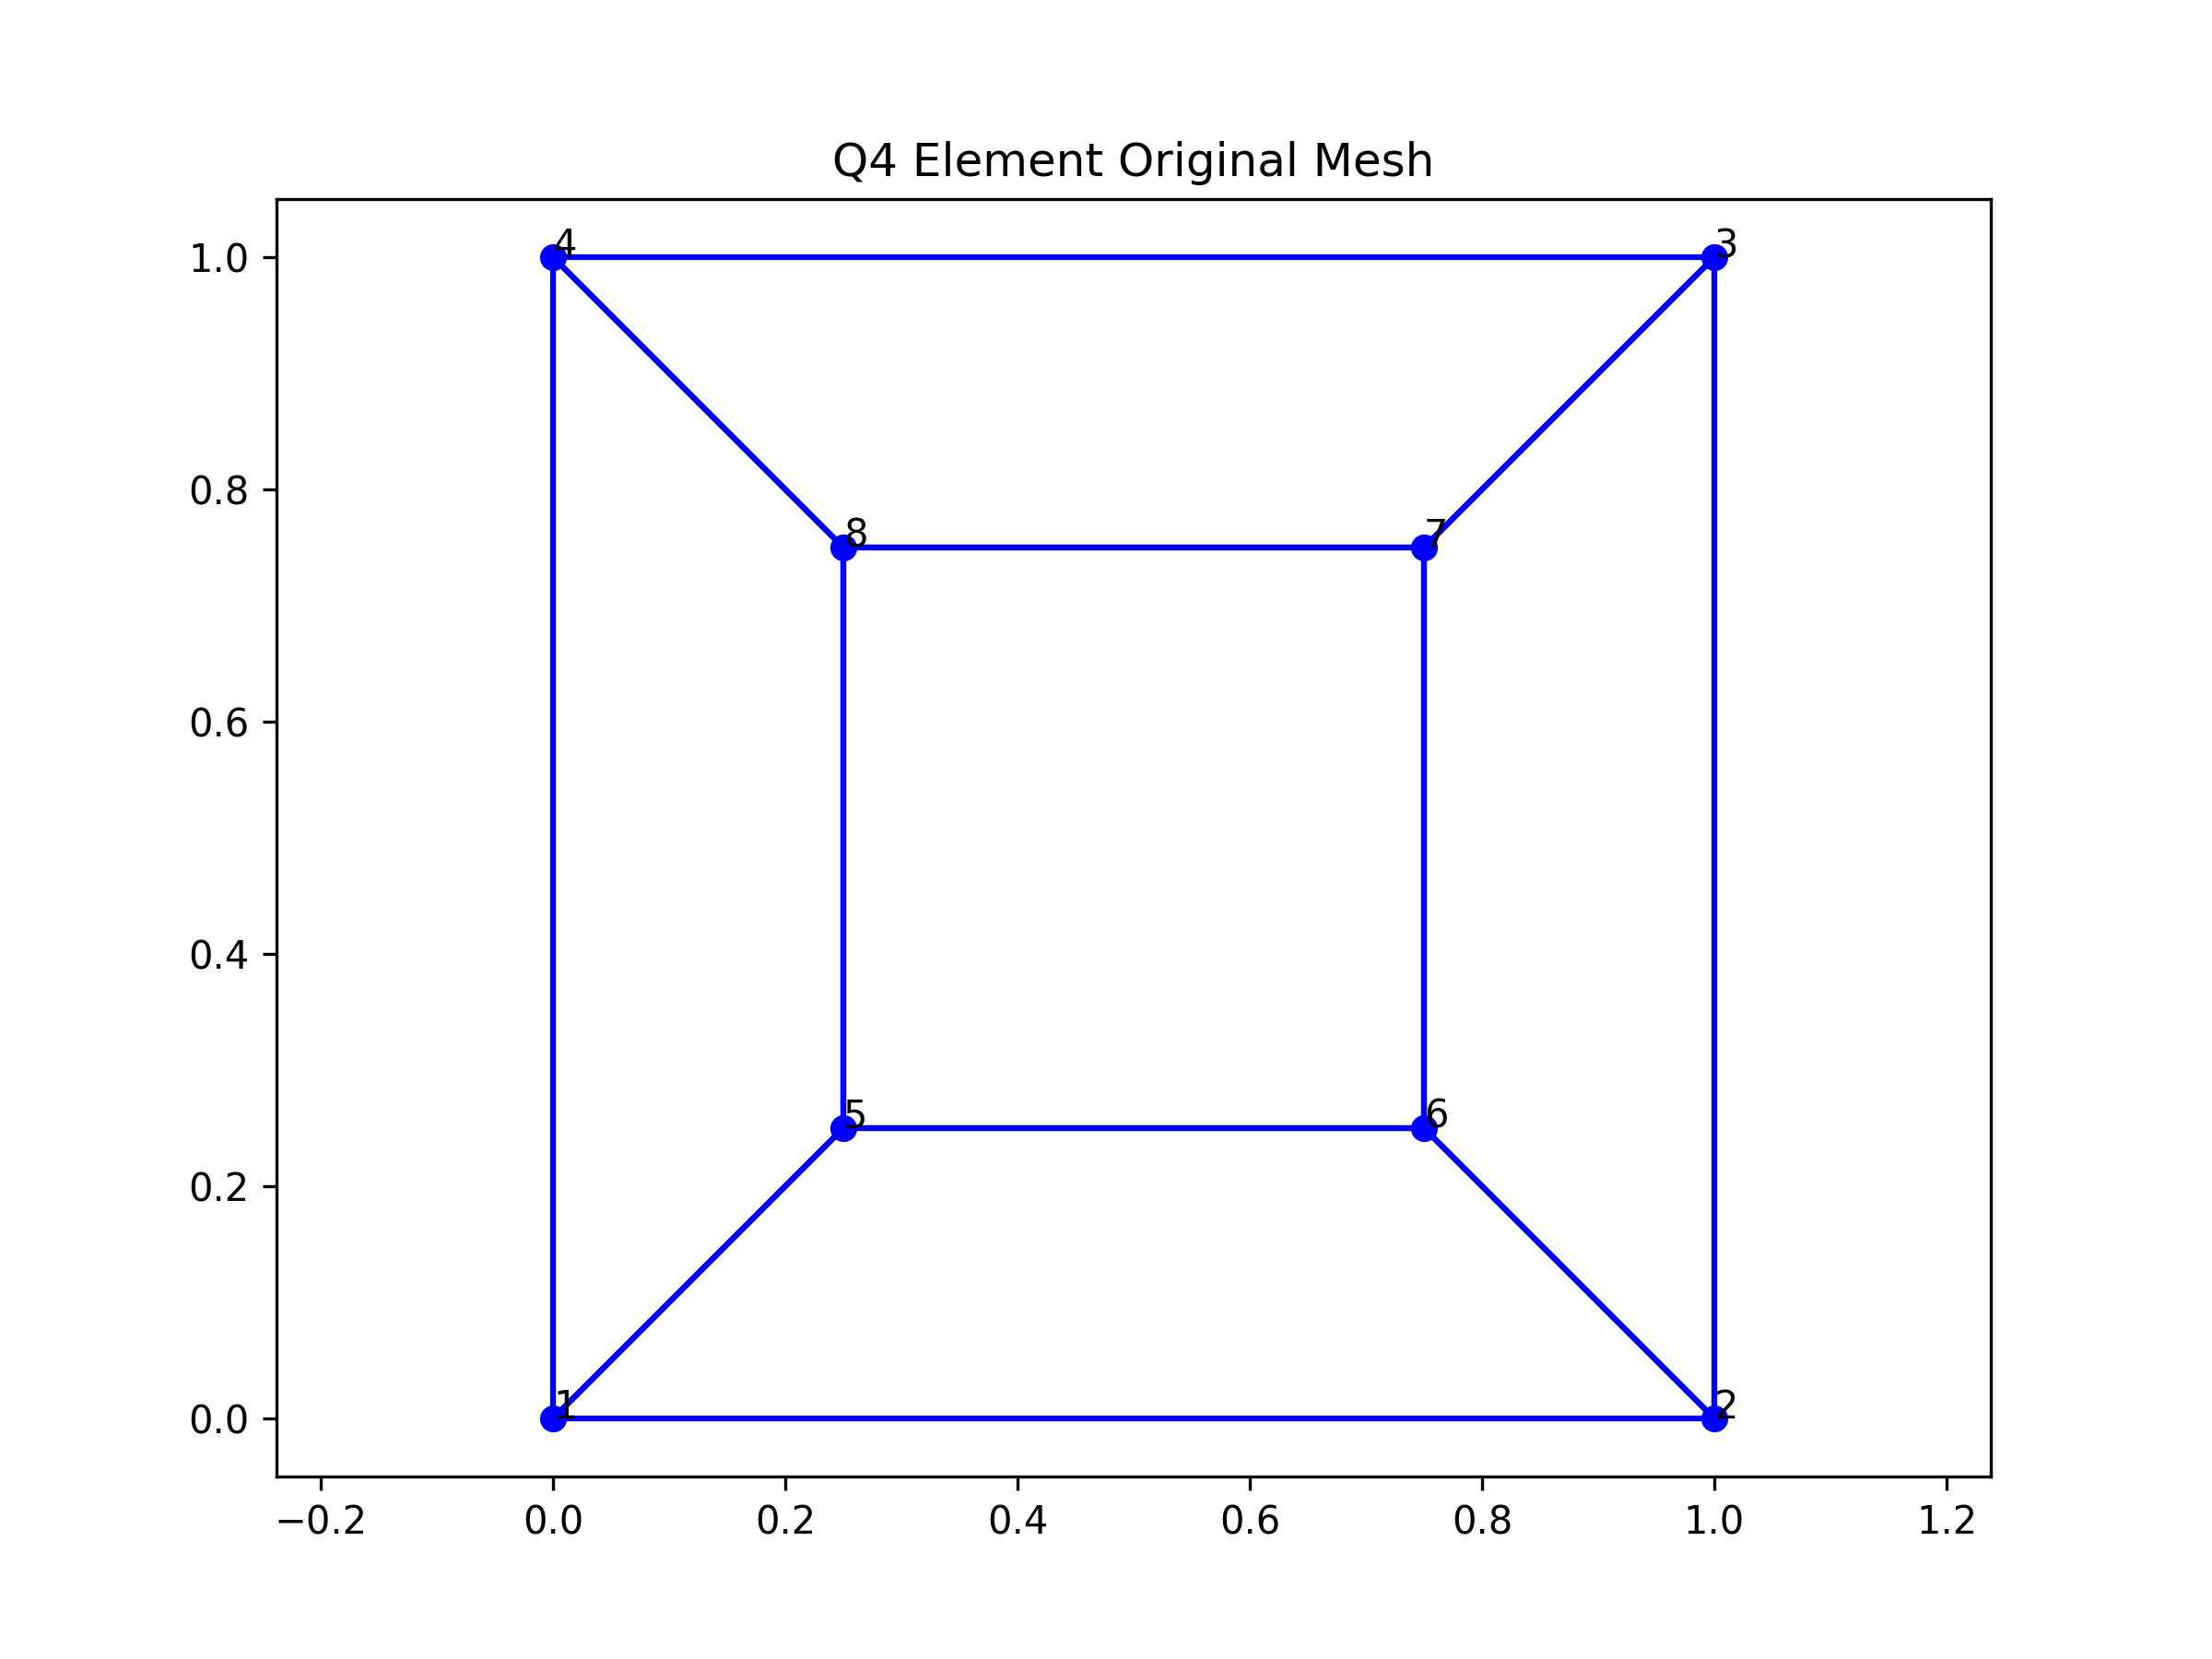
\includegraphics[width=0.6\textwidth]{test_patch_original.png}
    \caption{Q4 element original mesh }
    \label{fig:patch_test_original}
\end{figure}
\begin{figure}[htbp]
    \centering
    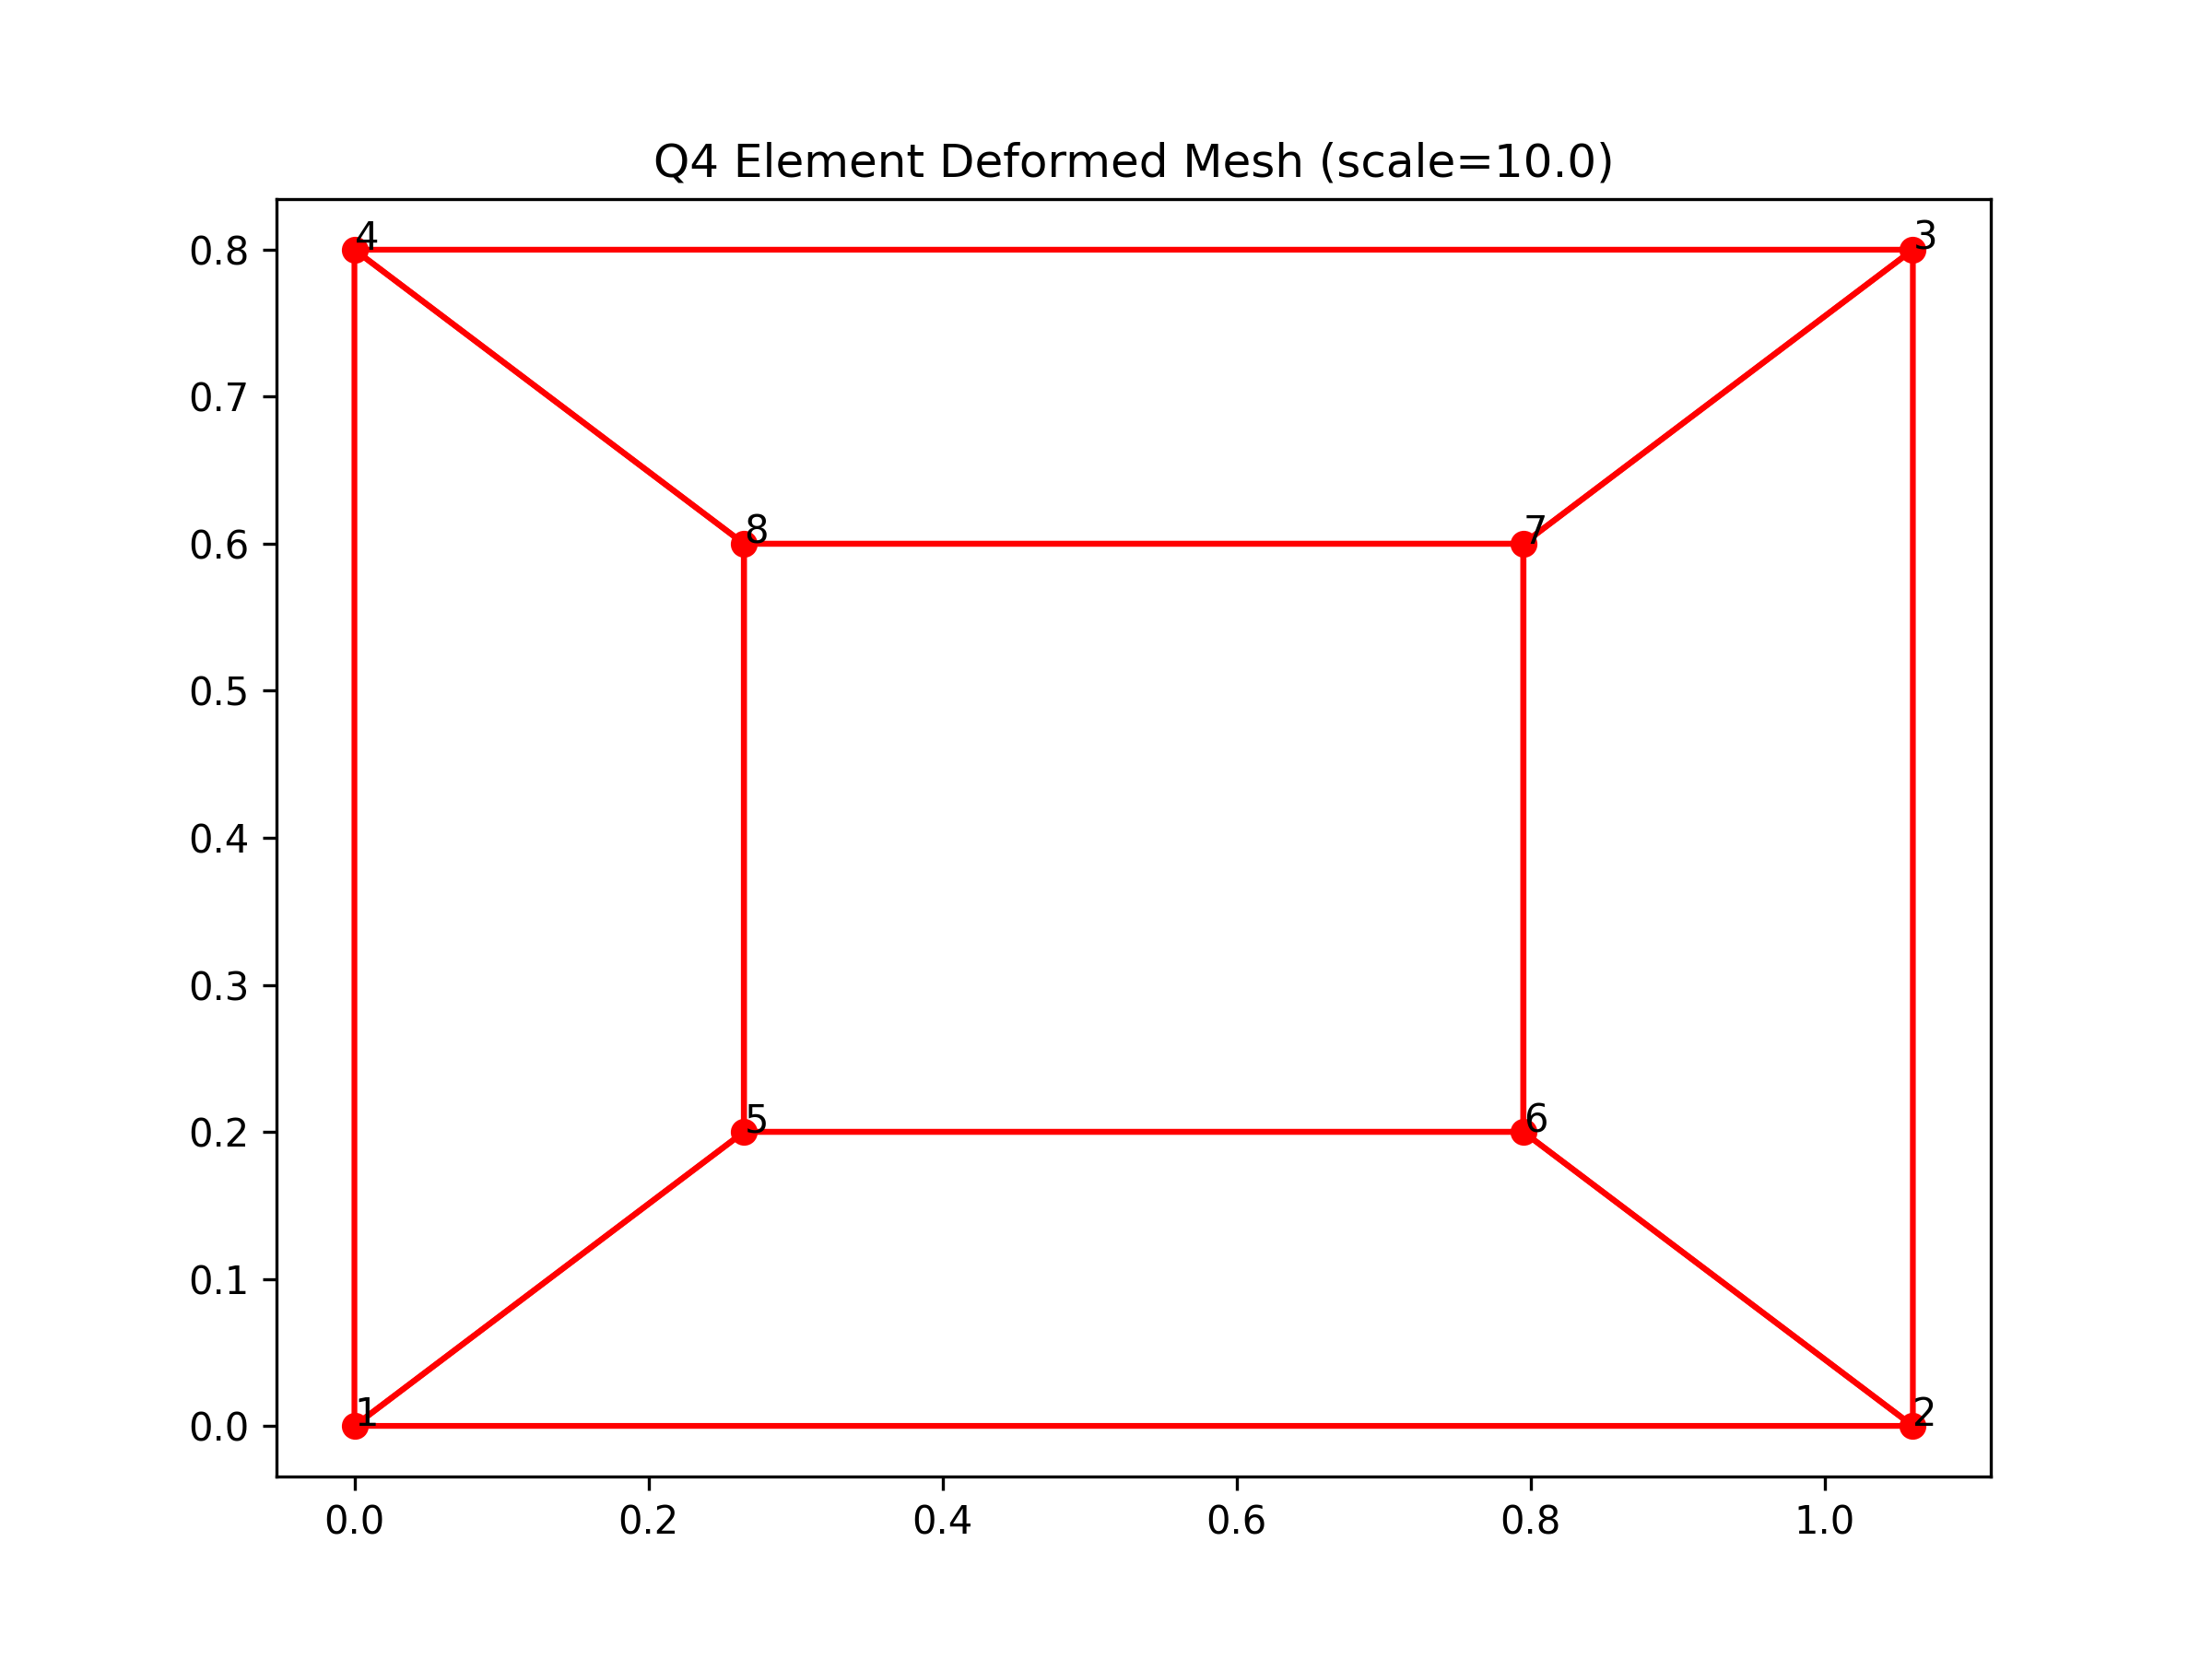
\includegraphics[width=0.6\textwidth]{test_patch_deformed.png}
    \caption{Q4 element deformed mesh (scale=10.0)}
    \label{fig:patch_test_deform}
\end{figure}
\section{Convergence test}
The convergence test is a crucial step in verifying the accuracy of the finite element method. It involves refining the mesh and observing how the solution converges to the exact solution as the mesh is refined.

\subsection{geometry}
A cantilever beam with dimensions 1×2 subjected to pure bending is adopted as a benchmark case for convergence analysis.
The details of the input file \texttt{test1\_2.dat} have already been given in an earlier section.

\subsection{Visualization of results}

\begin{figure}[htbp]
    \centering
    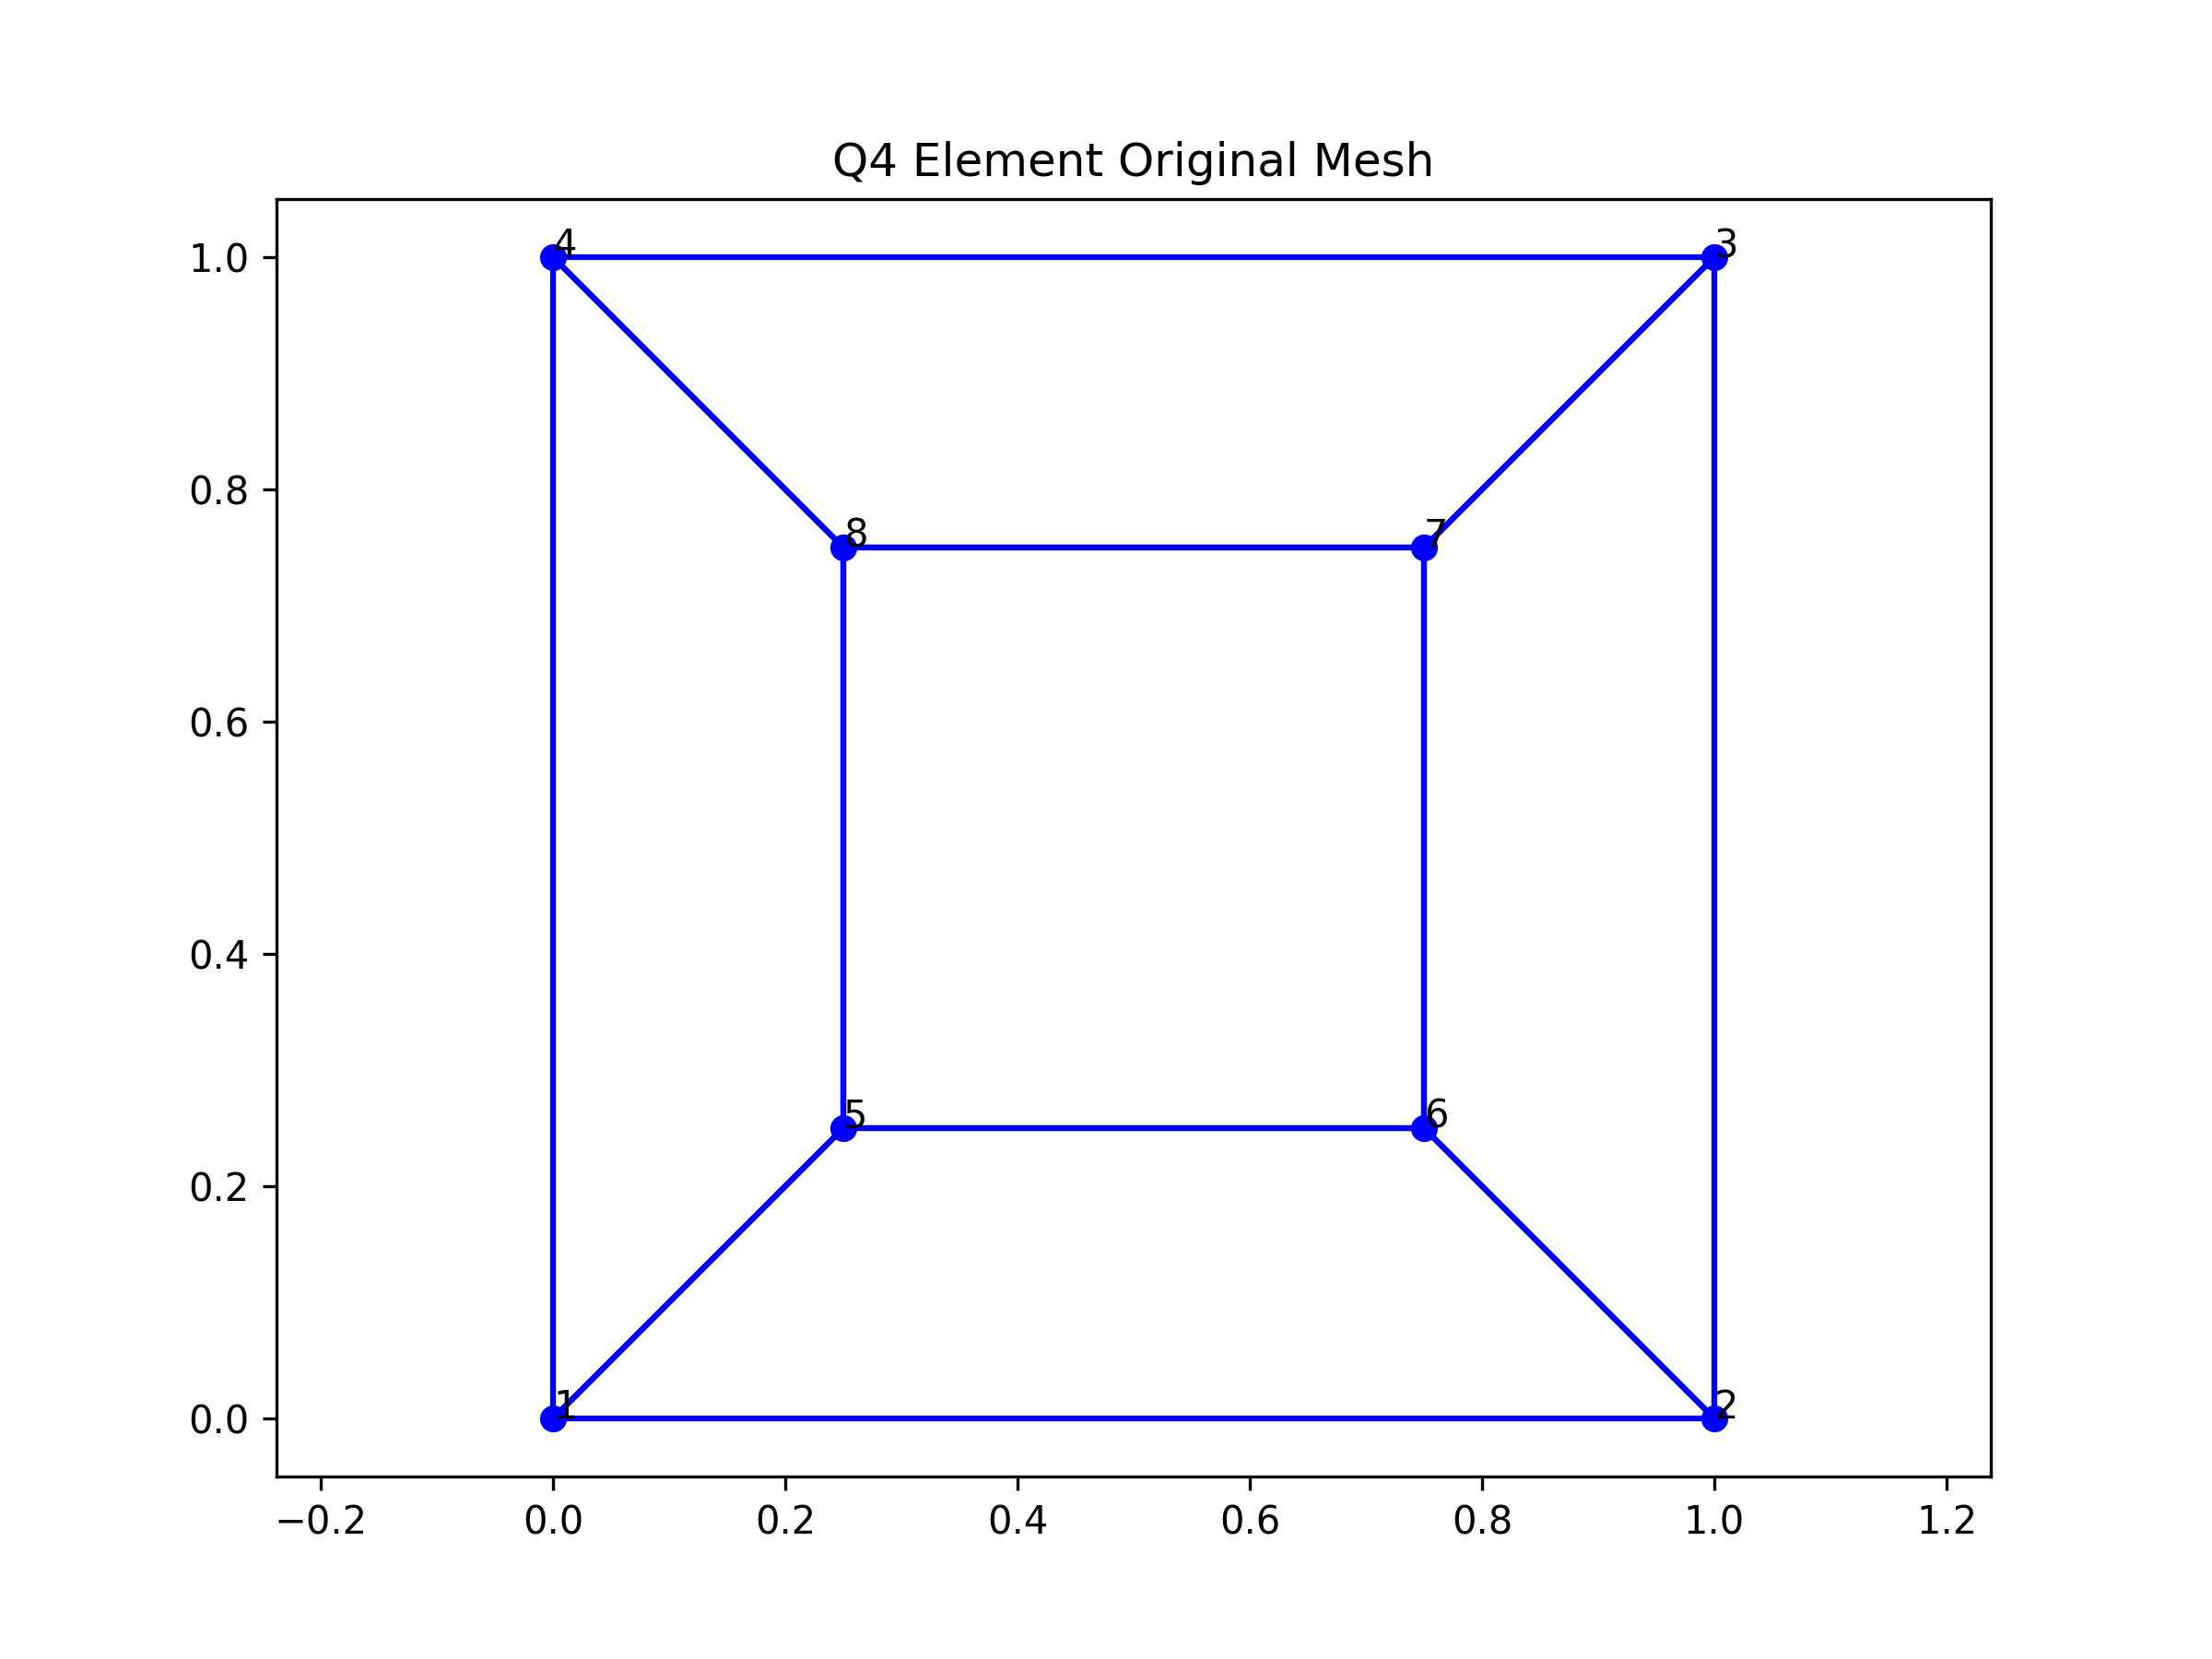
\includegraphics[width=0.6\textwidth]{test_patch_original.png}
    \caption{Q4 element original mesh }
    \label{fig:patch1_2_original}
\end{figure}

\begin{figure}[htbp]
    \centering
    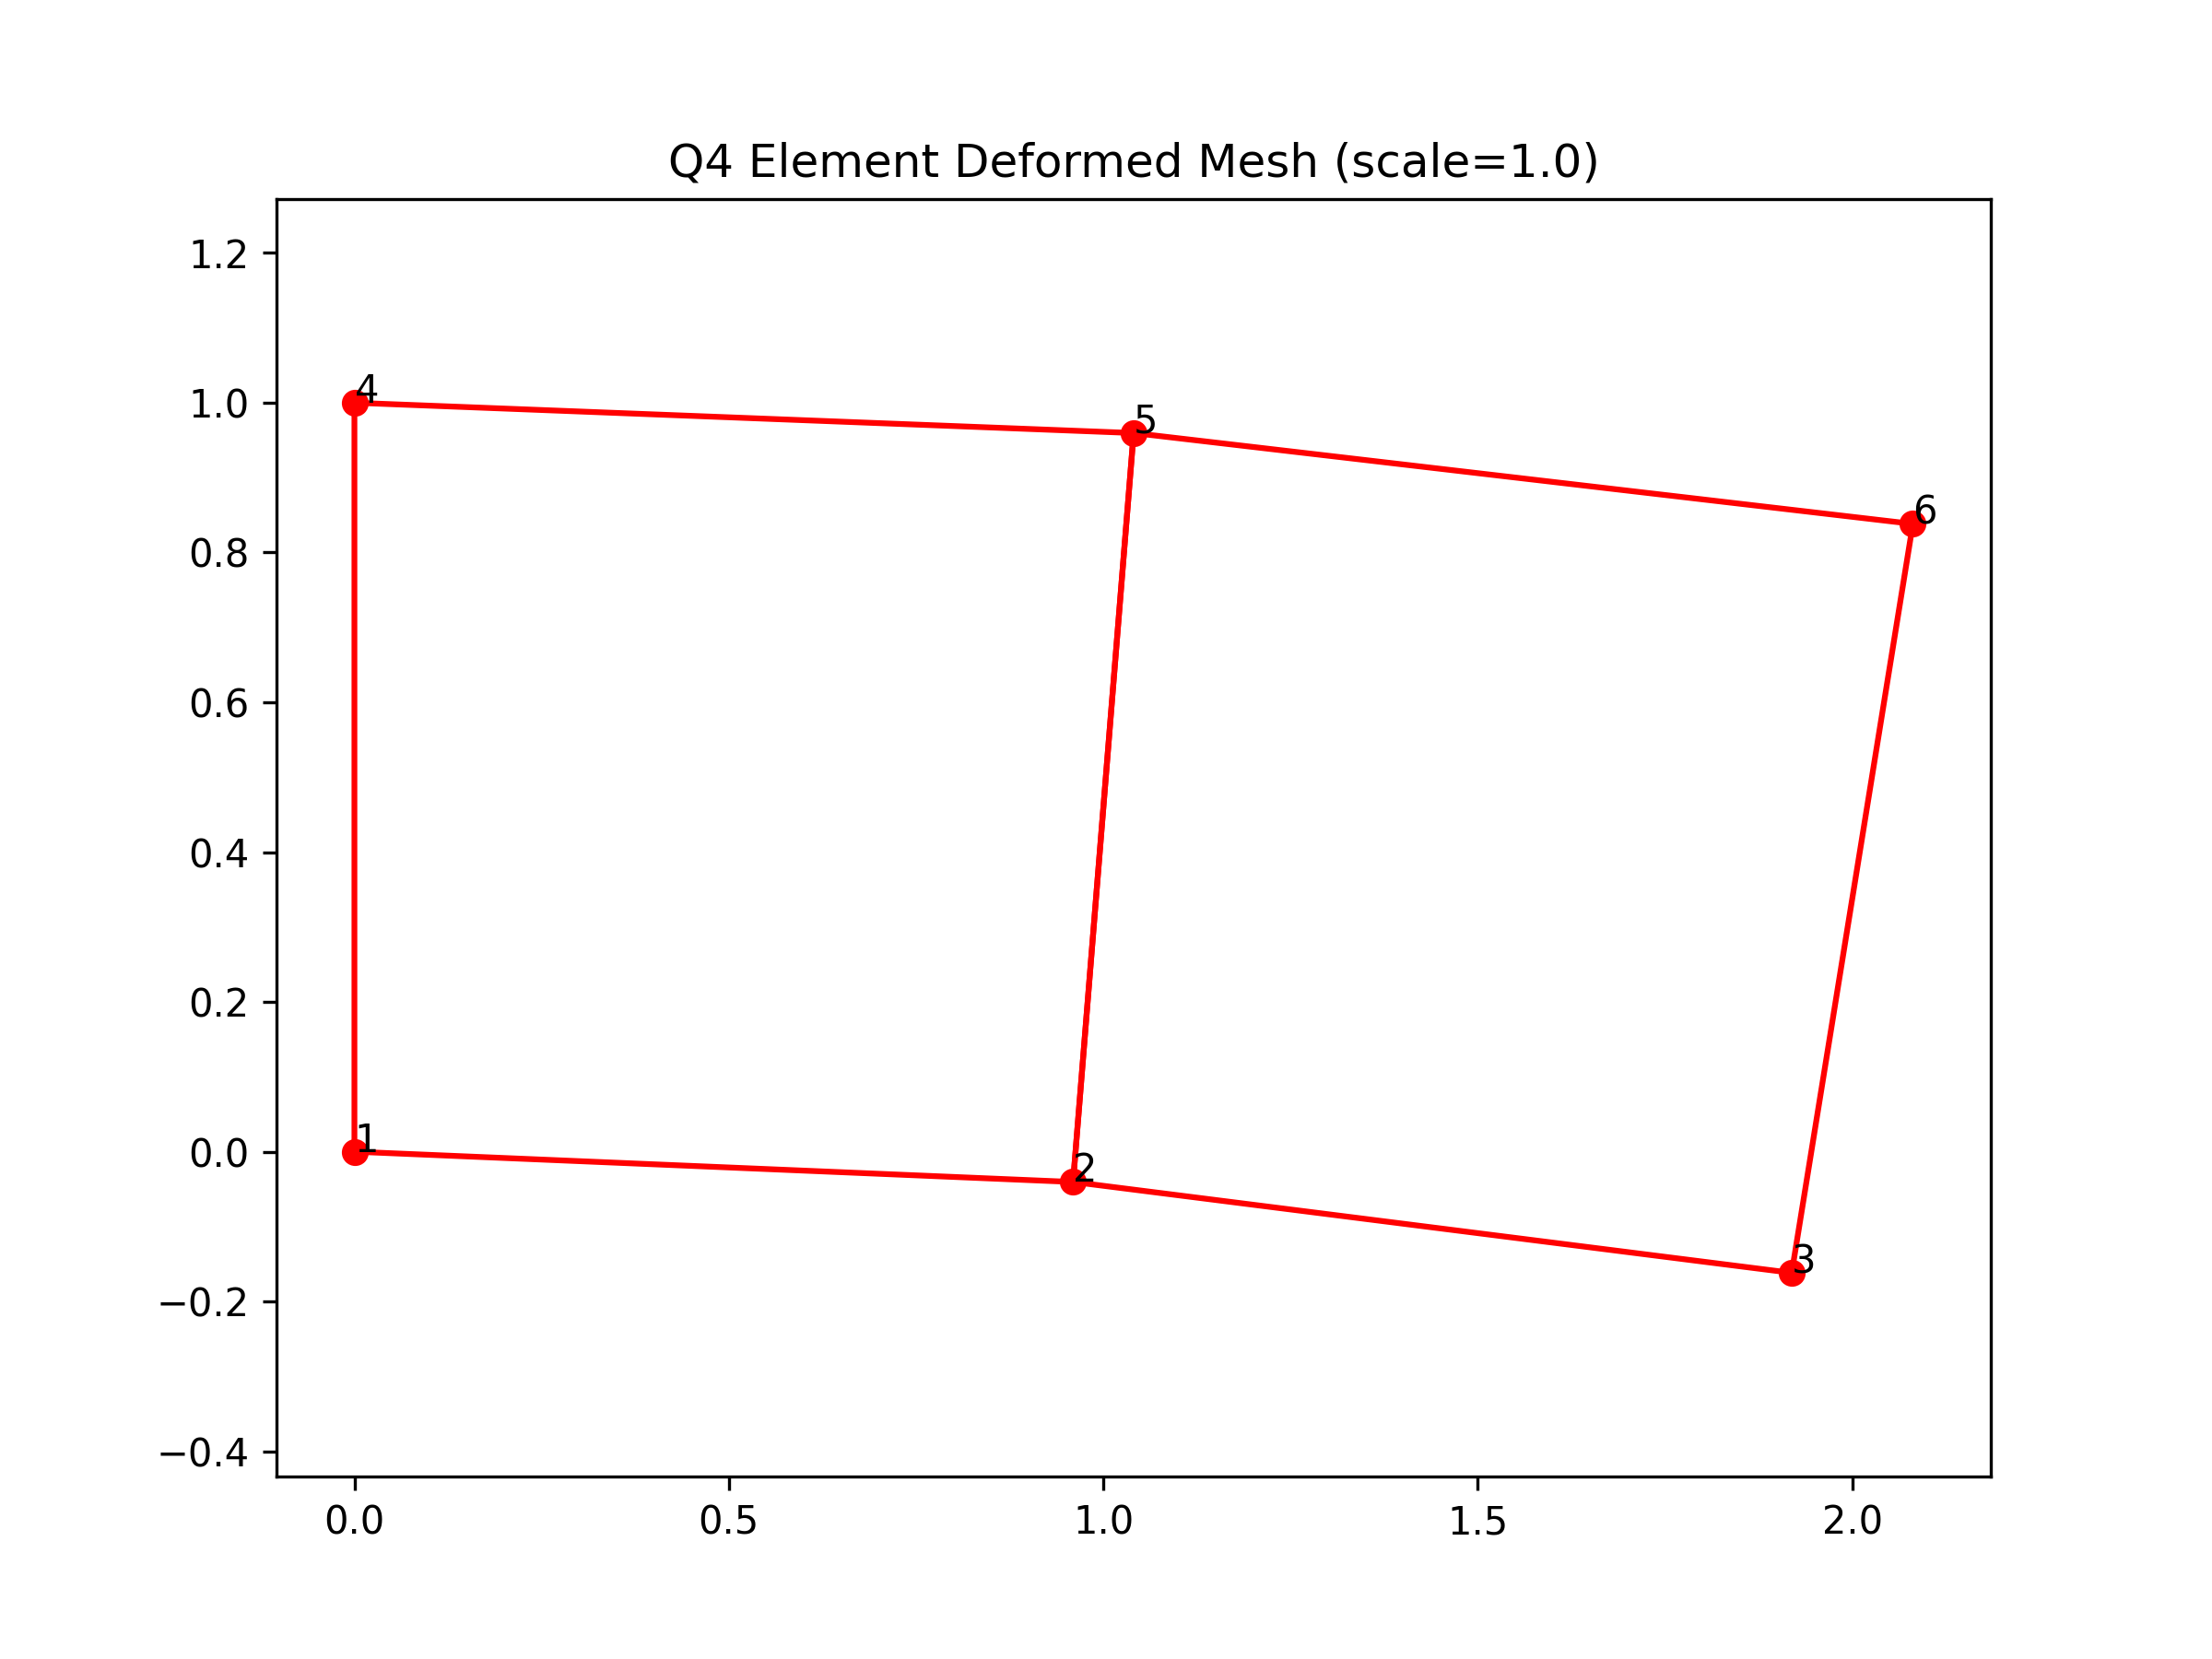
\includegraphics[width=0.6\textwidth]{test1_2_deformed.png}
    \caption{Q4 element deformed mesh (scale=10.0)}
    \label{fig:patch1_2_deform}
\end{figure}

\begin{figure}[htbp]
    \centering
    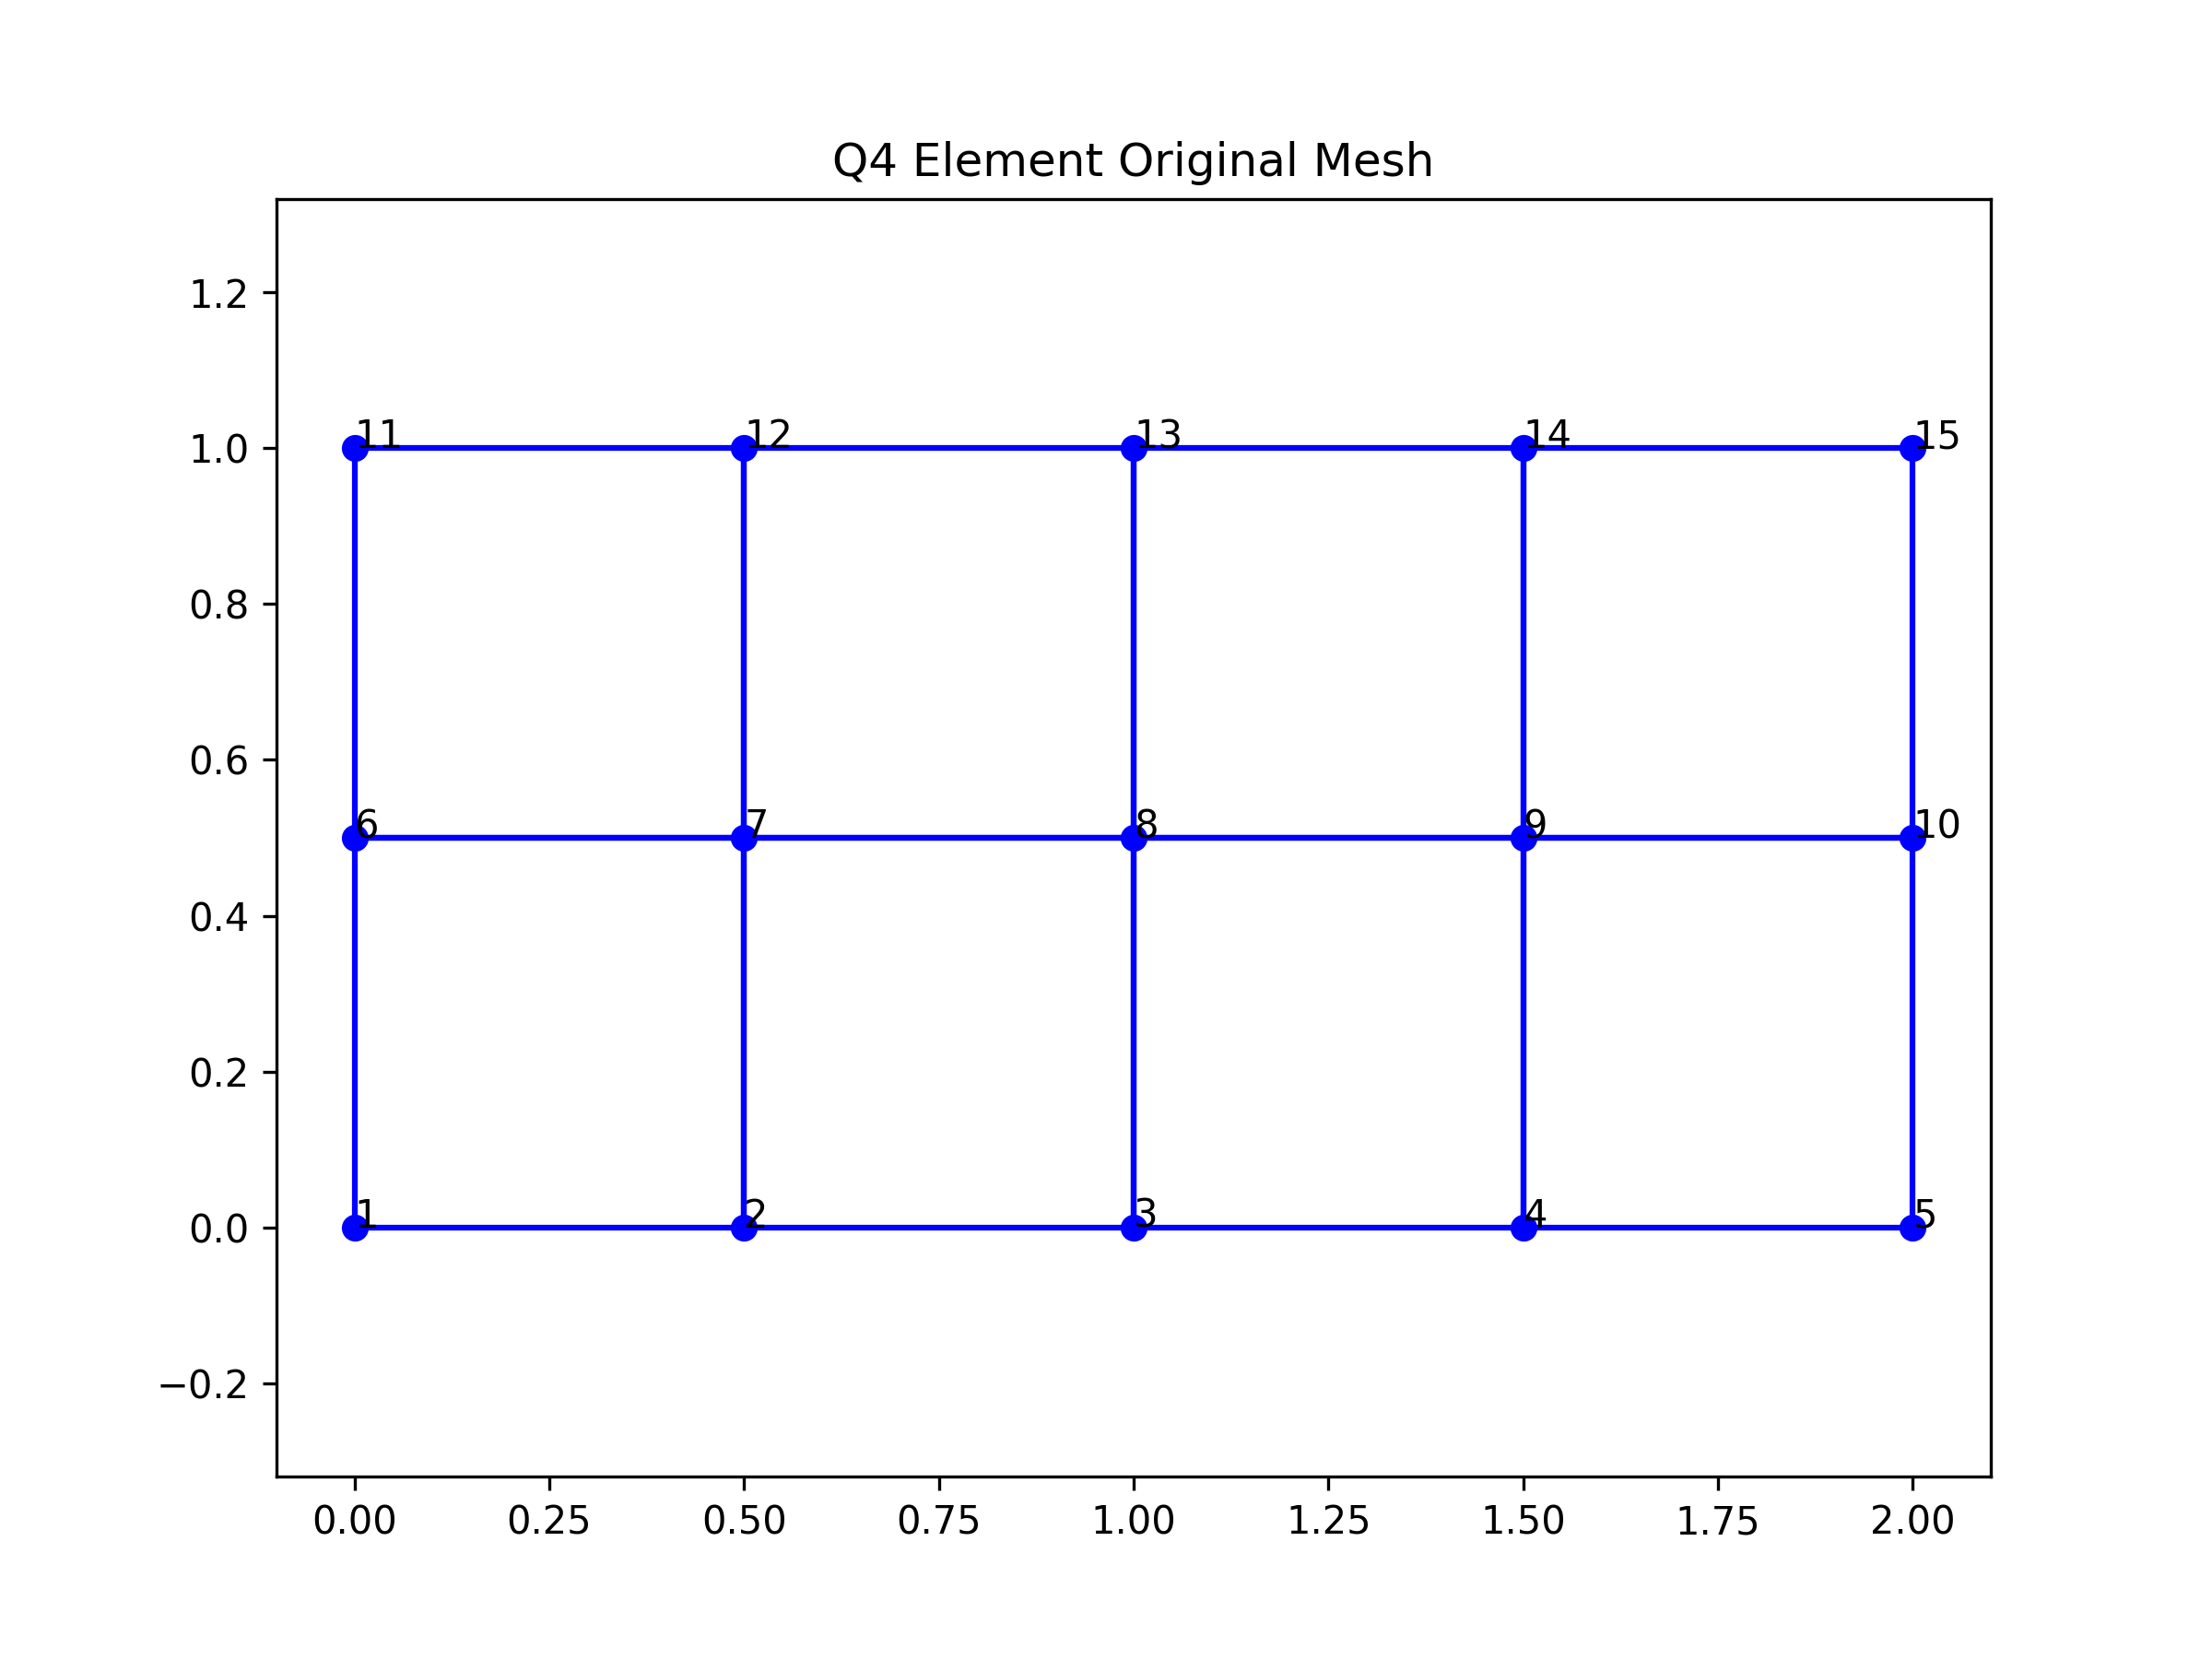
\includegraphics[width=0.6\textwidth]{test2_4_original.png}
    \caption{Q4 element original mesh }
    \label{fig:patch2_4_original}
\end{figure}

\begin{figure}[htbp]
    \centering
    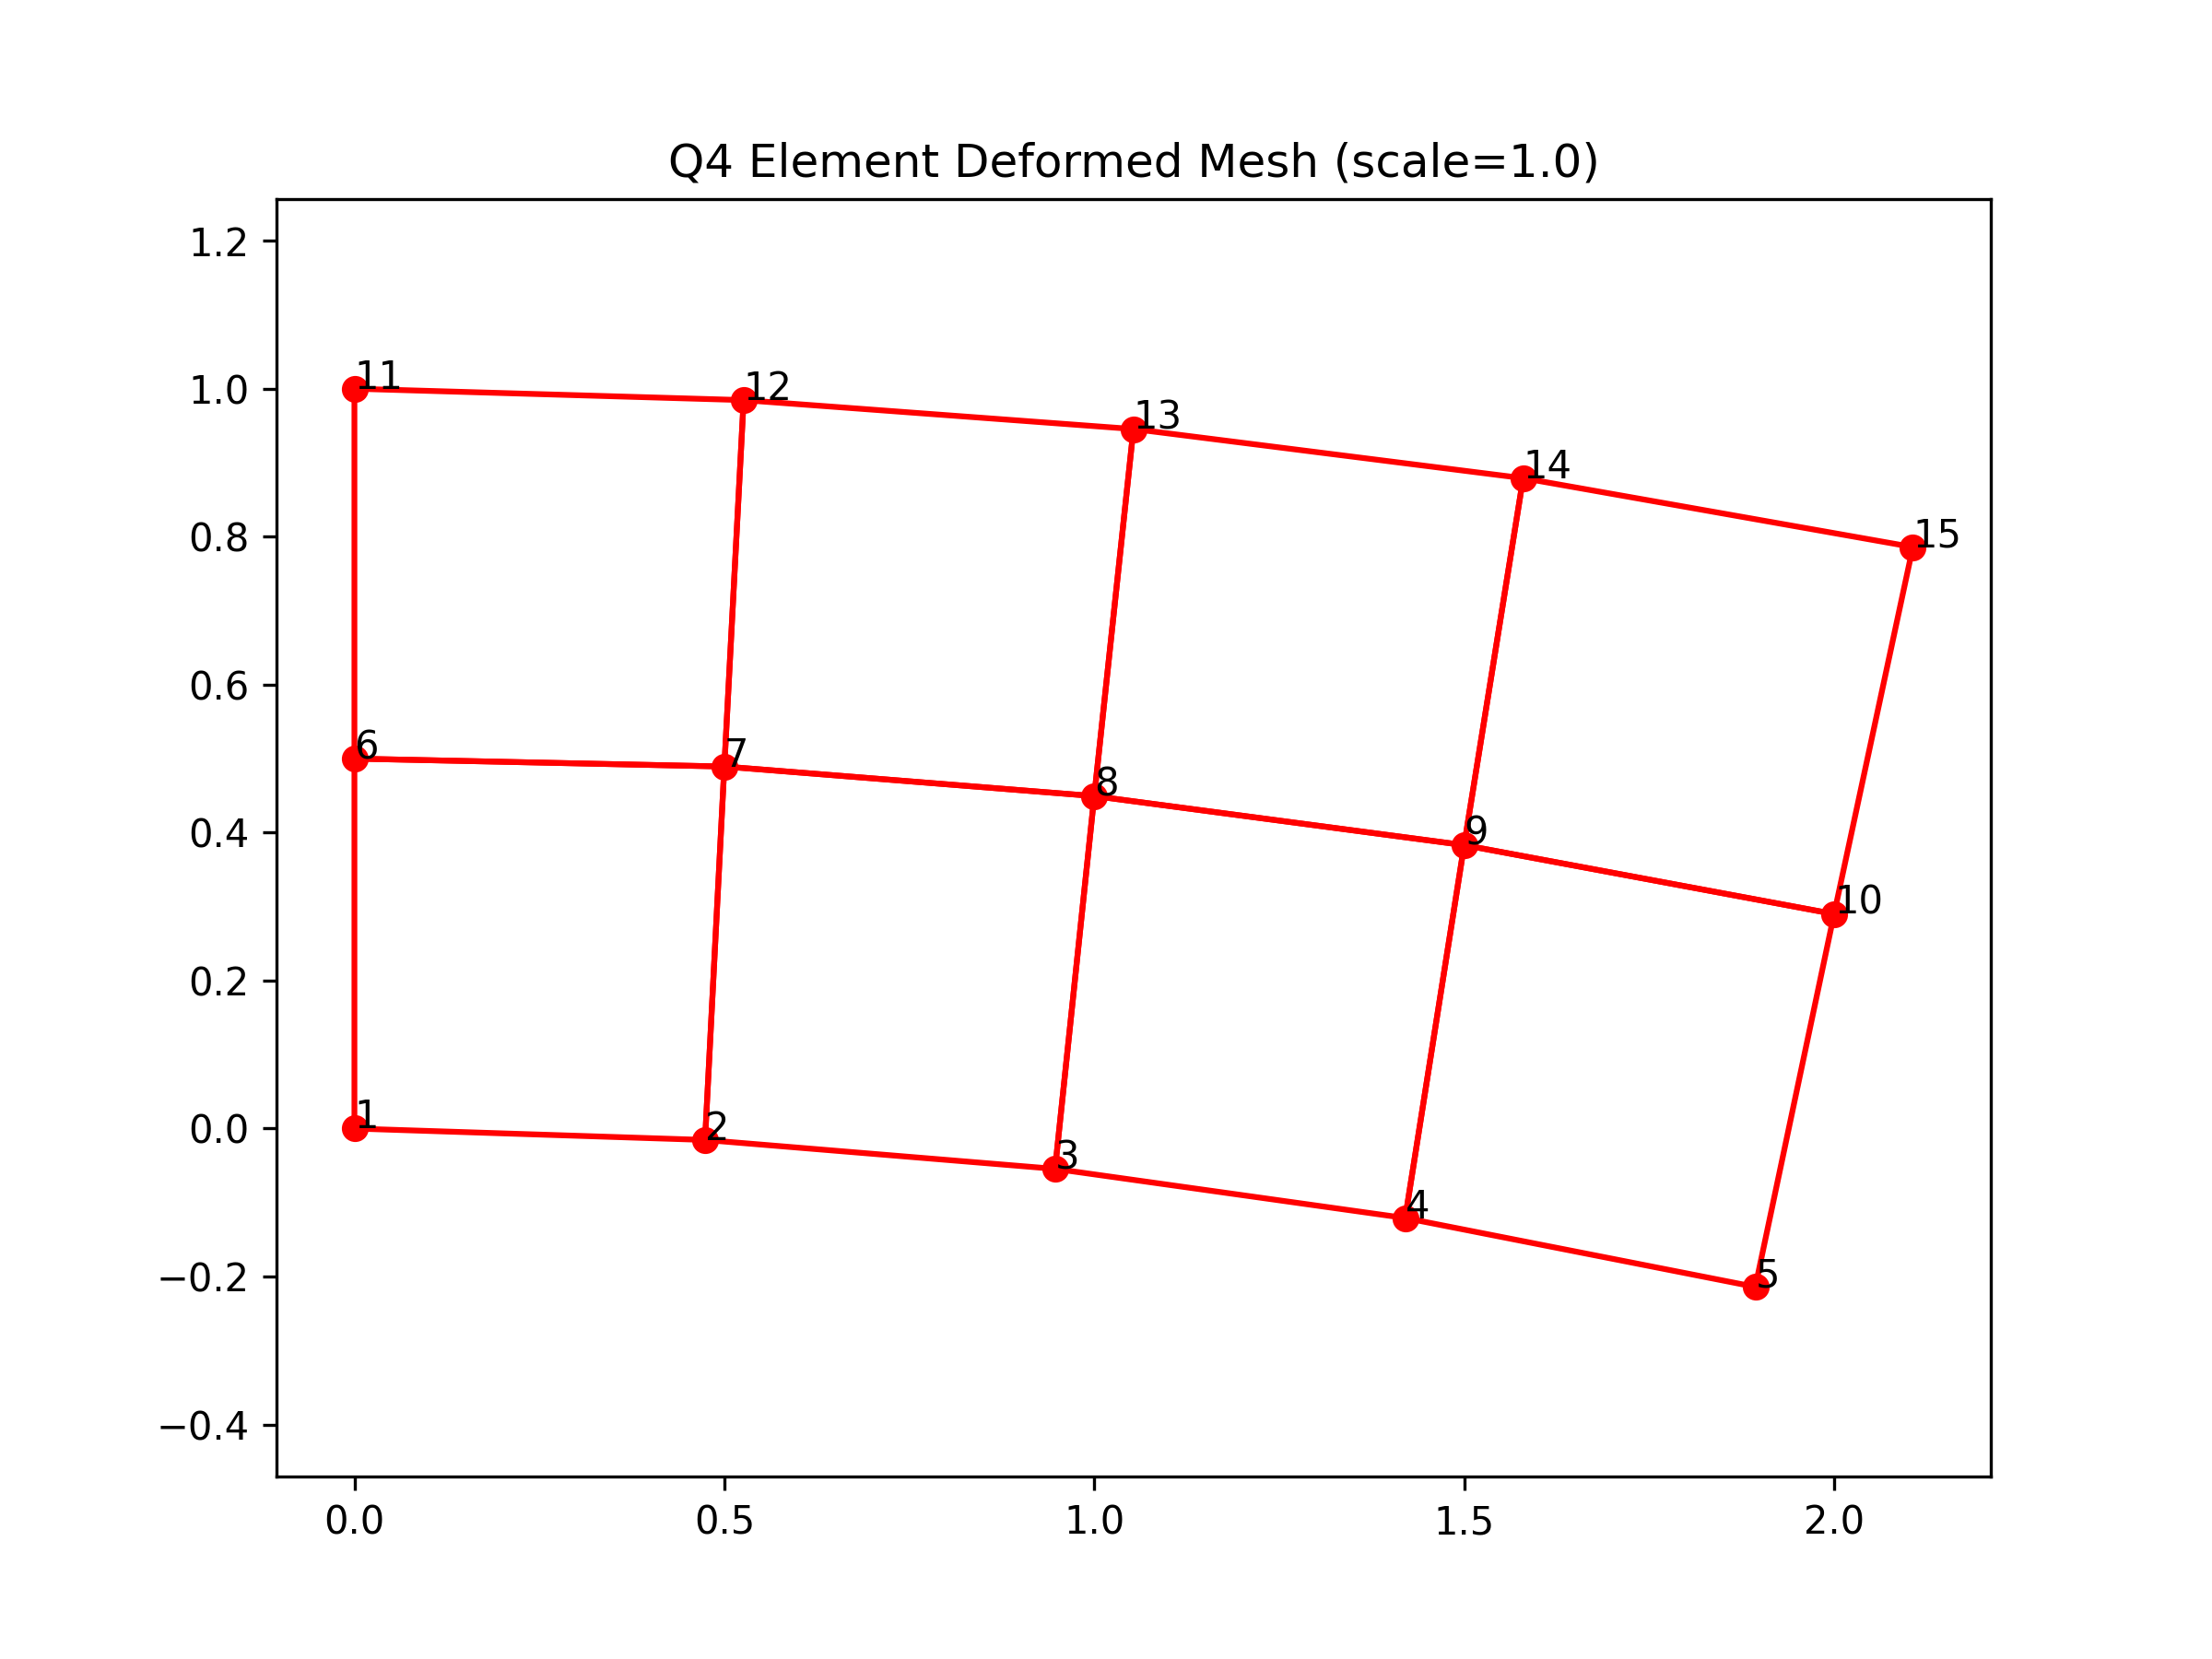
\includegraphics[width=0.6\textwidth]{test2_4_deformed.png}
    \caption{Q4 element deformed mesh (scale=10.0)}
    \label{fig:patch2_4_deform}
\end{figure}

\begin{figure}[htbp]
    \centering
    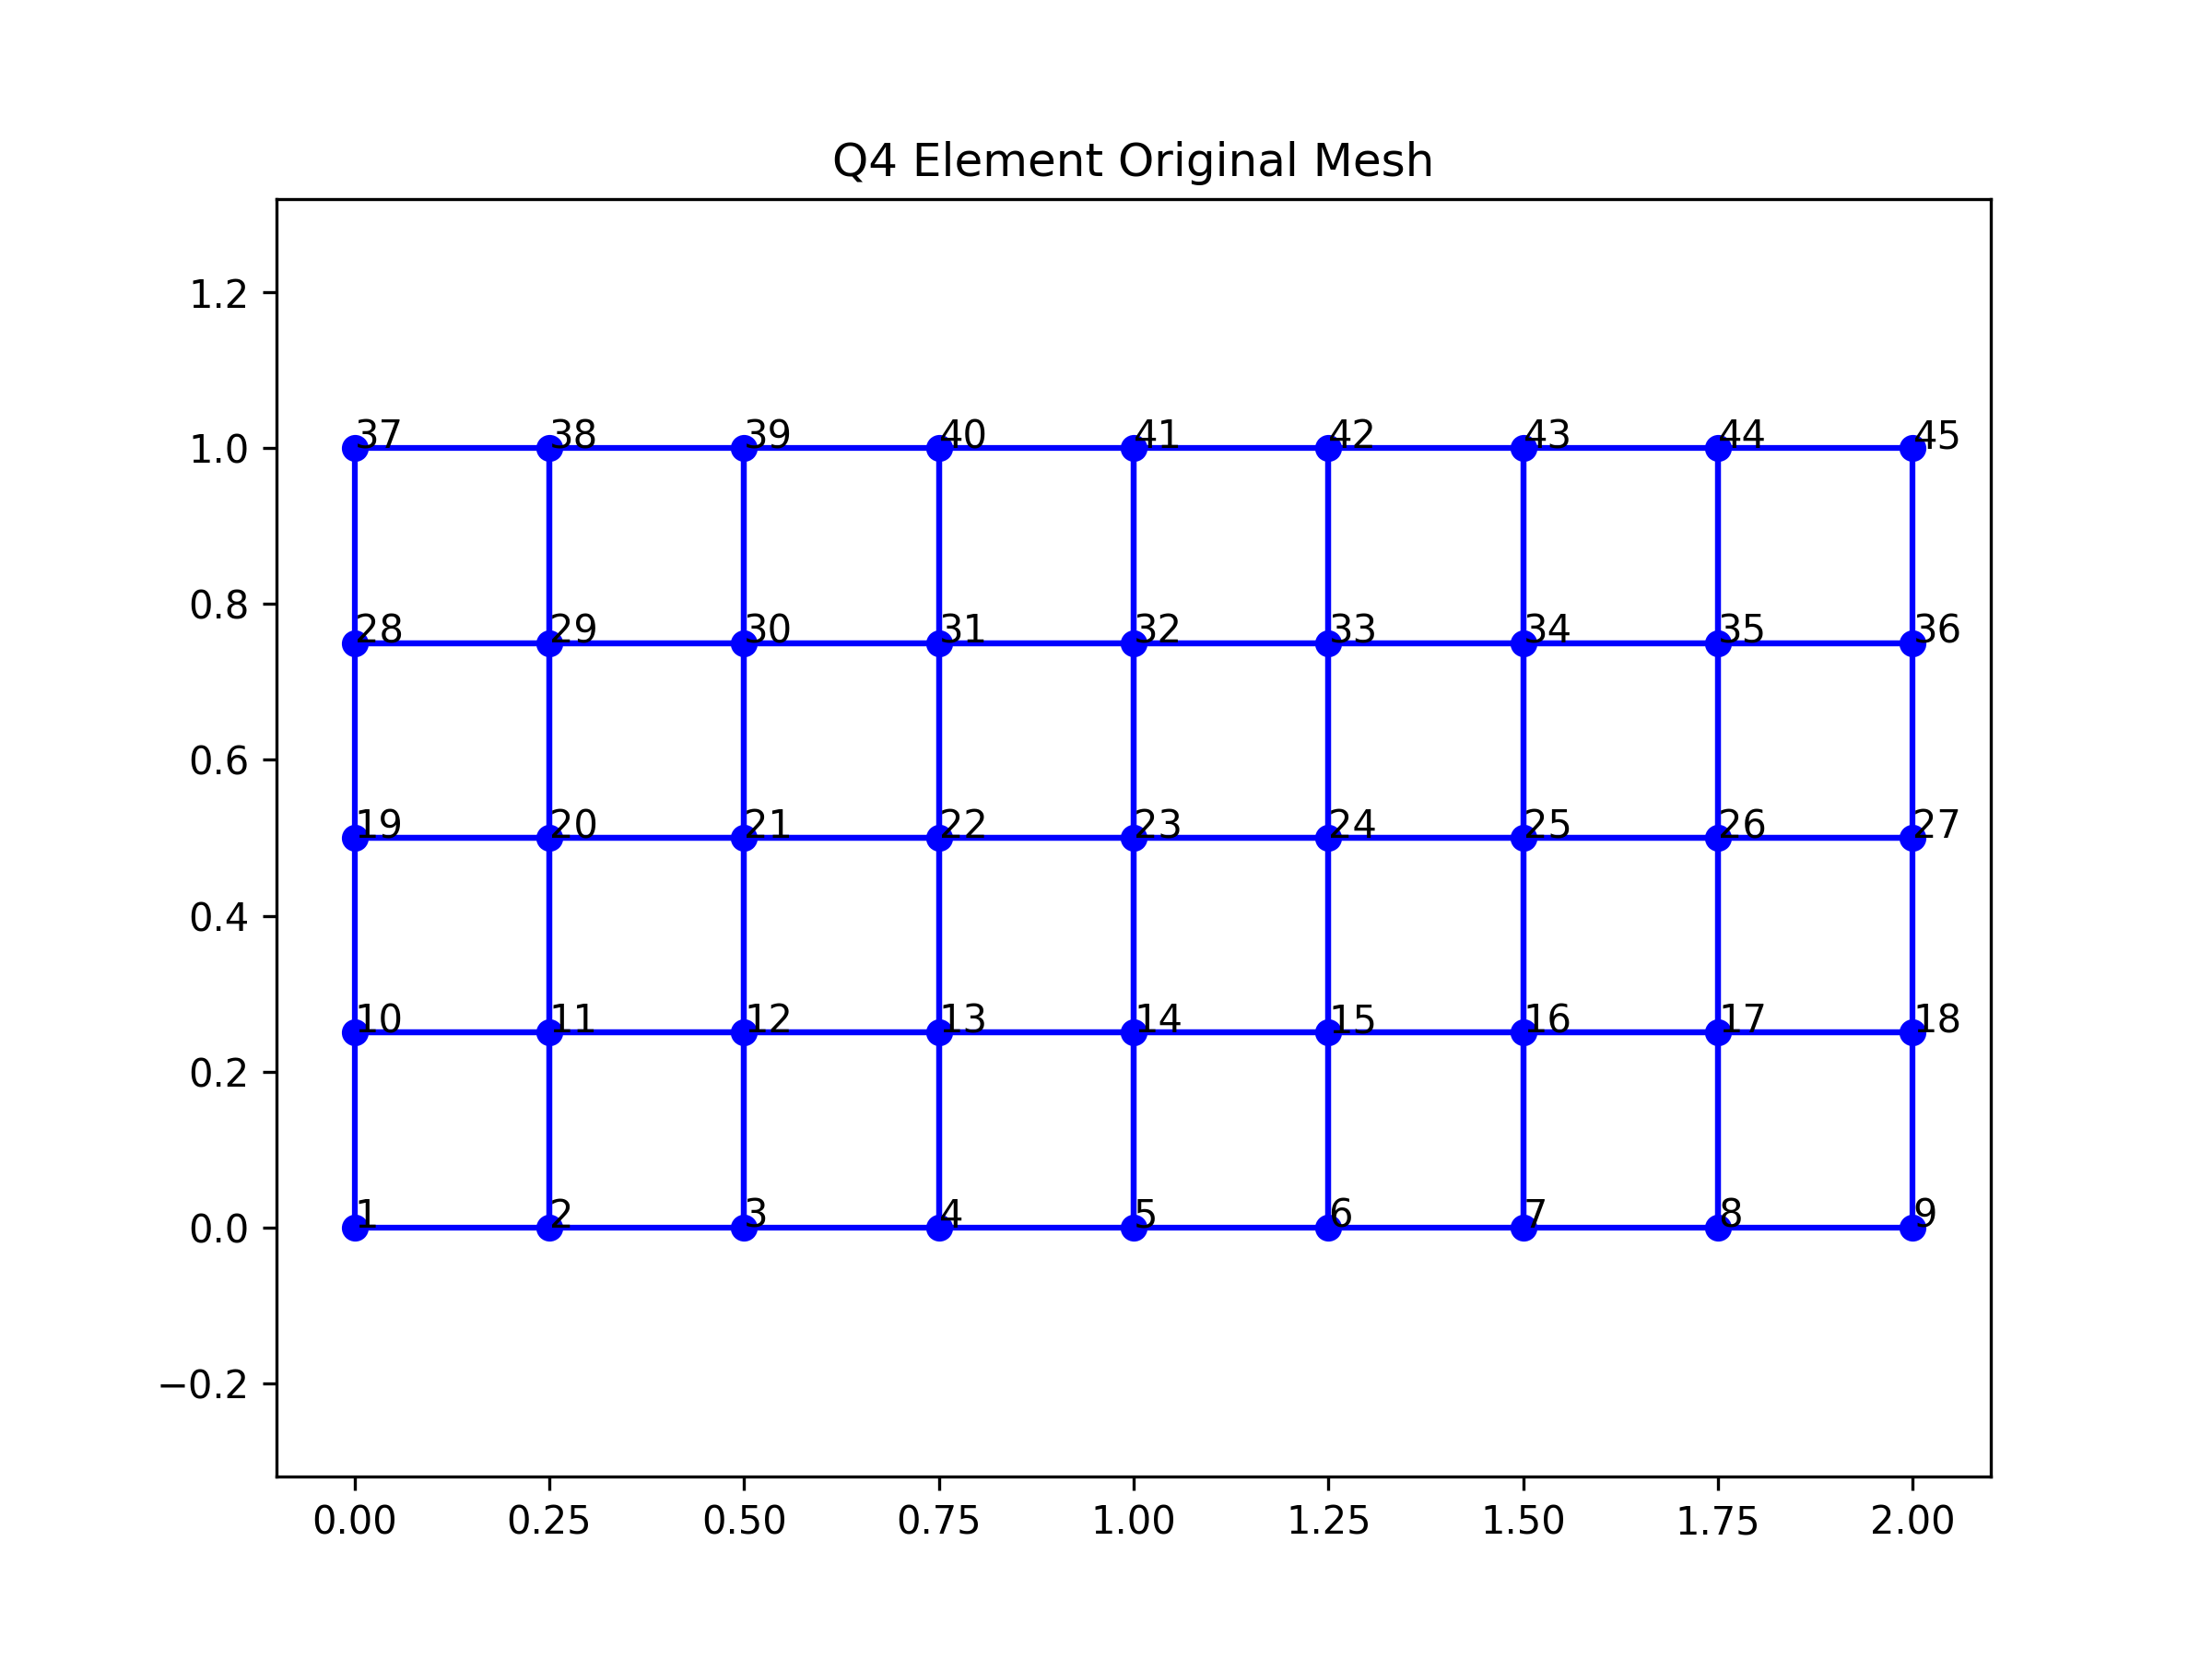
\includegraphics[width=0.6\textwidth]{test4_8_original.png}
    \caption{Q4 element original mesh }
    \label{fig:patch4_8_original}
\end{figure}

\begin{figure}[htbp]
    \centering
    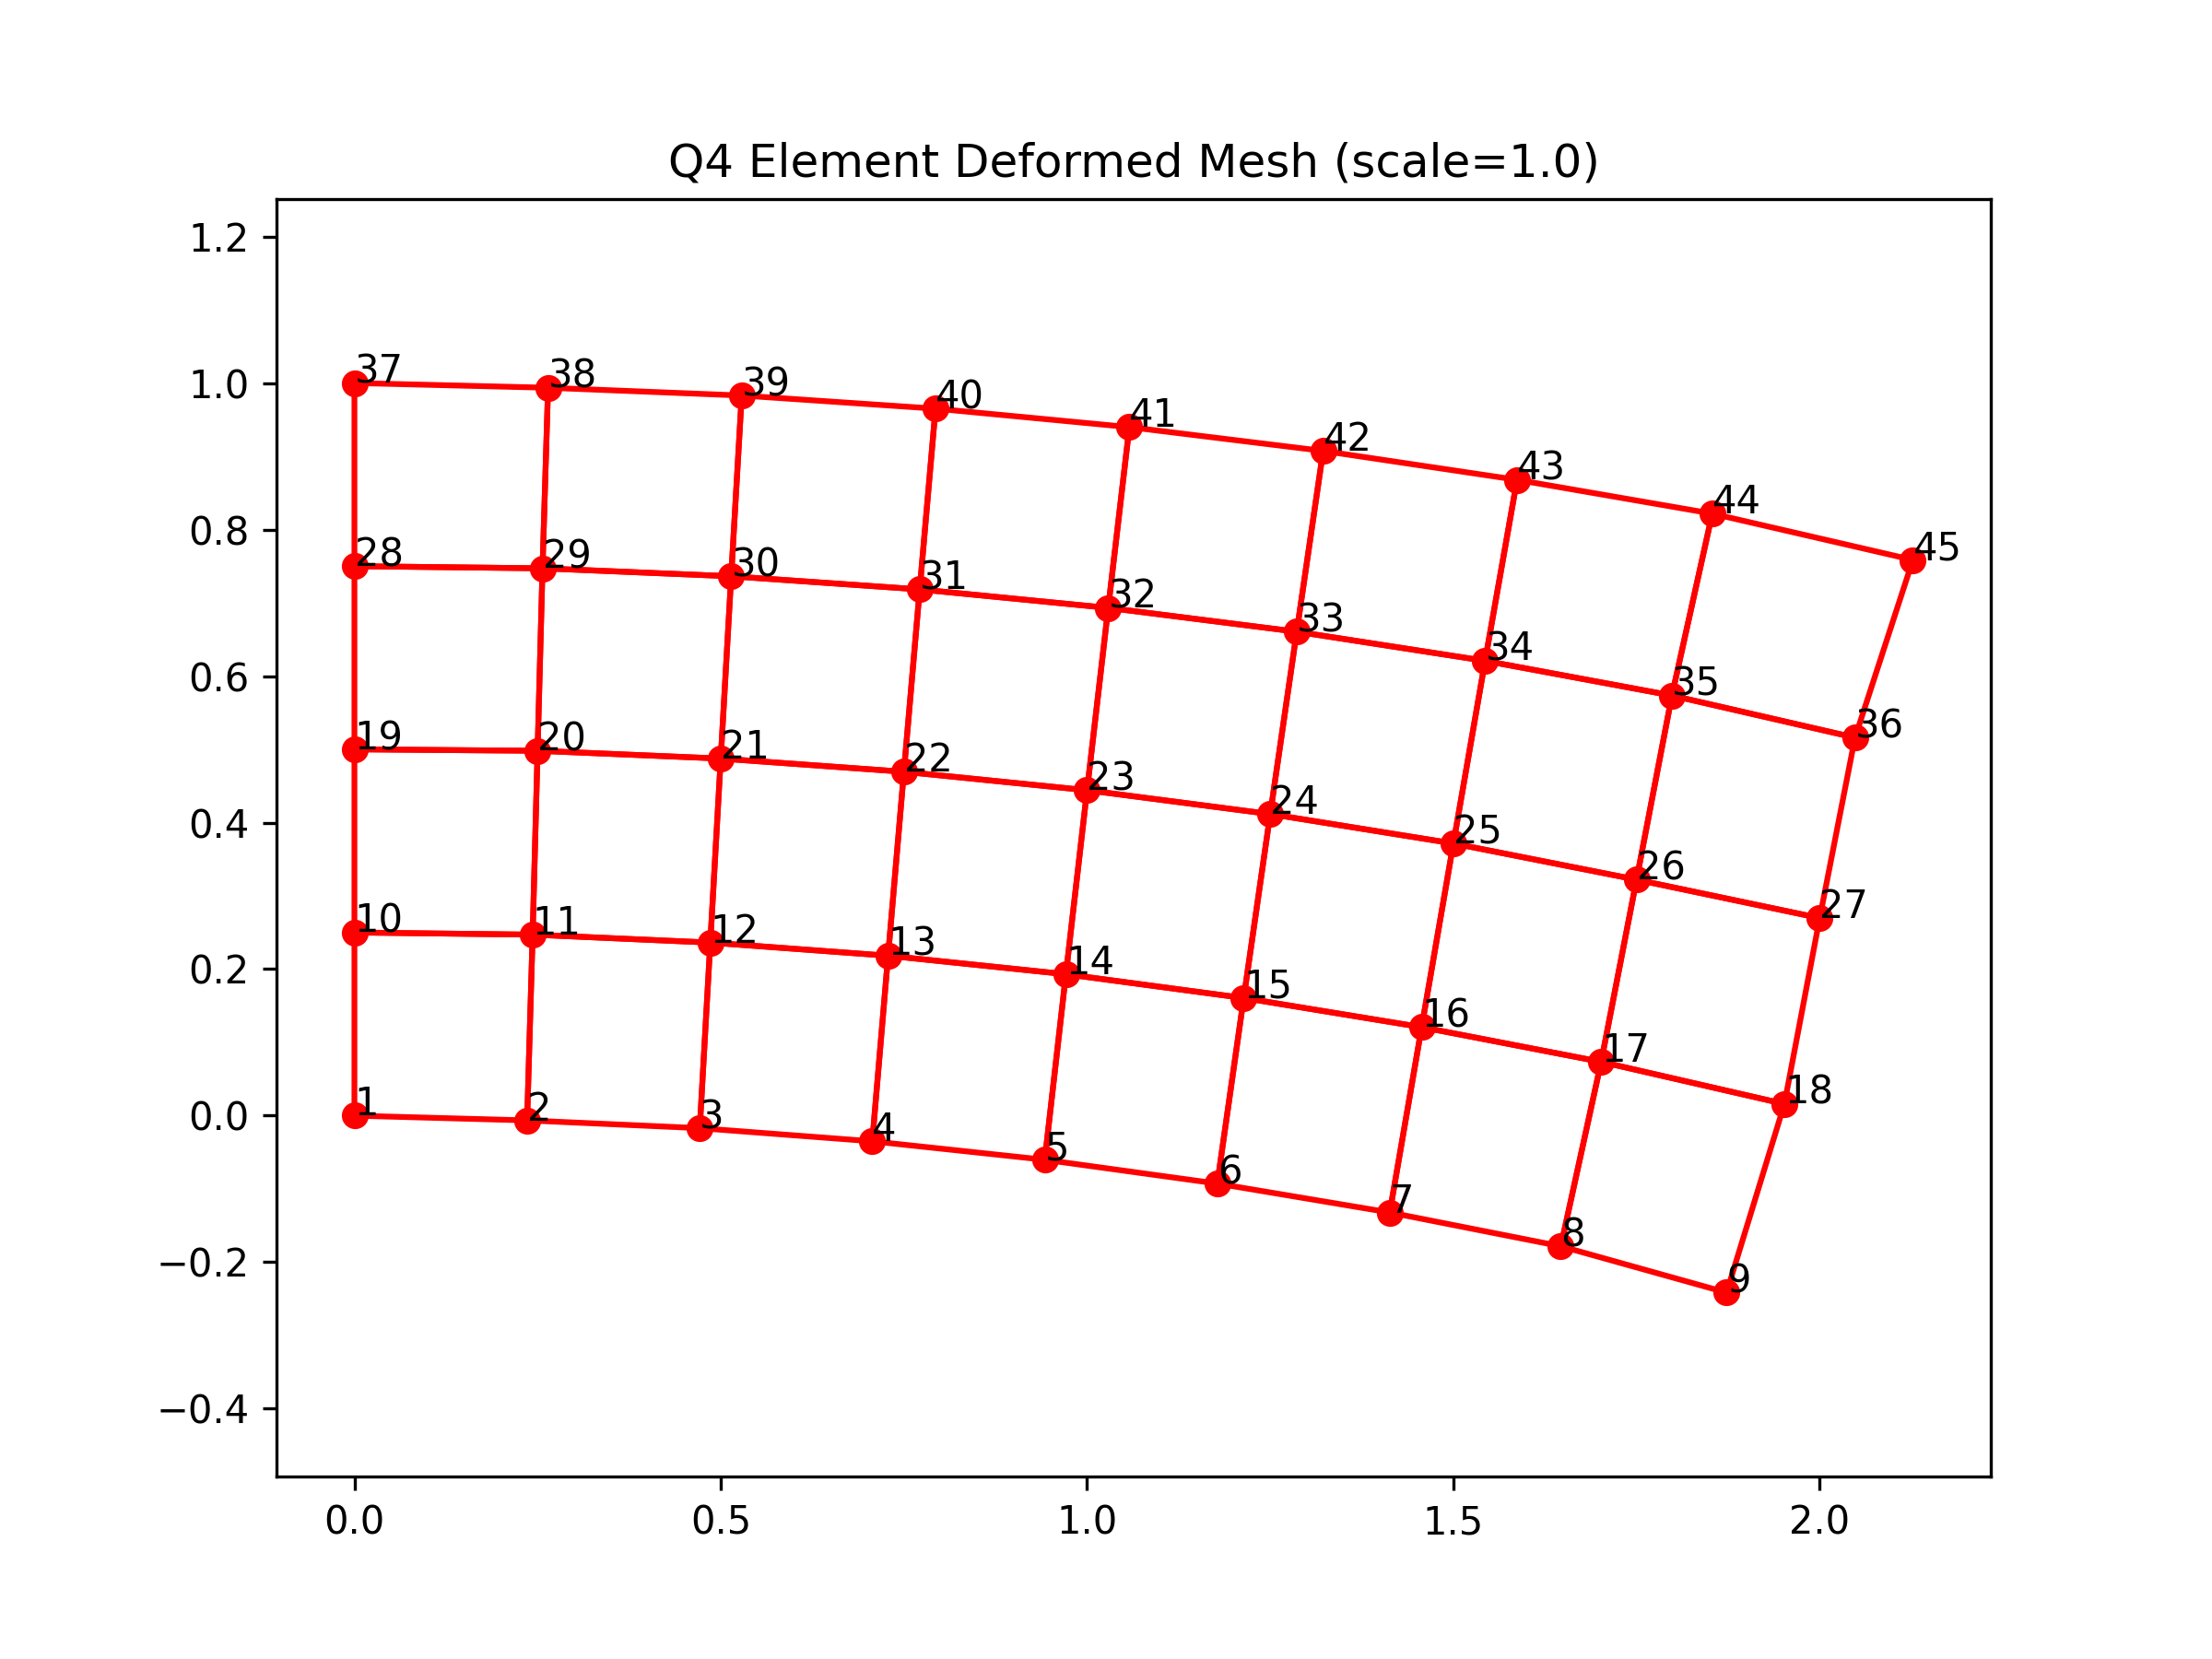
\includegraphics[width=0.6\textwidth]{test4_8_deformed.png}
    \caption{Q4 element deformed mesh (scale=10.0)}
    \label{fig:patch4_8_deform}\
\end{figure}

Compute the $L^2$ error norm and plot a log-log graph against the mesh size $h$. The resulting slope (convergence rate) is 1.693807741234391,
by using convergence.py and plotL2.py.

\begin{figure}[htbp]
    \centering
    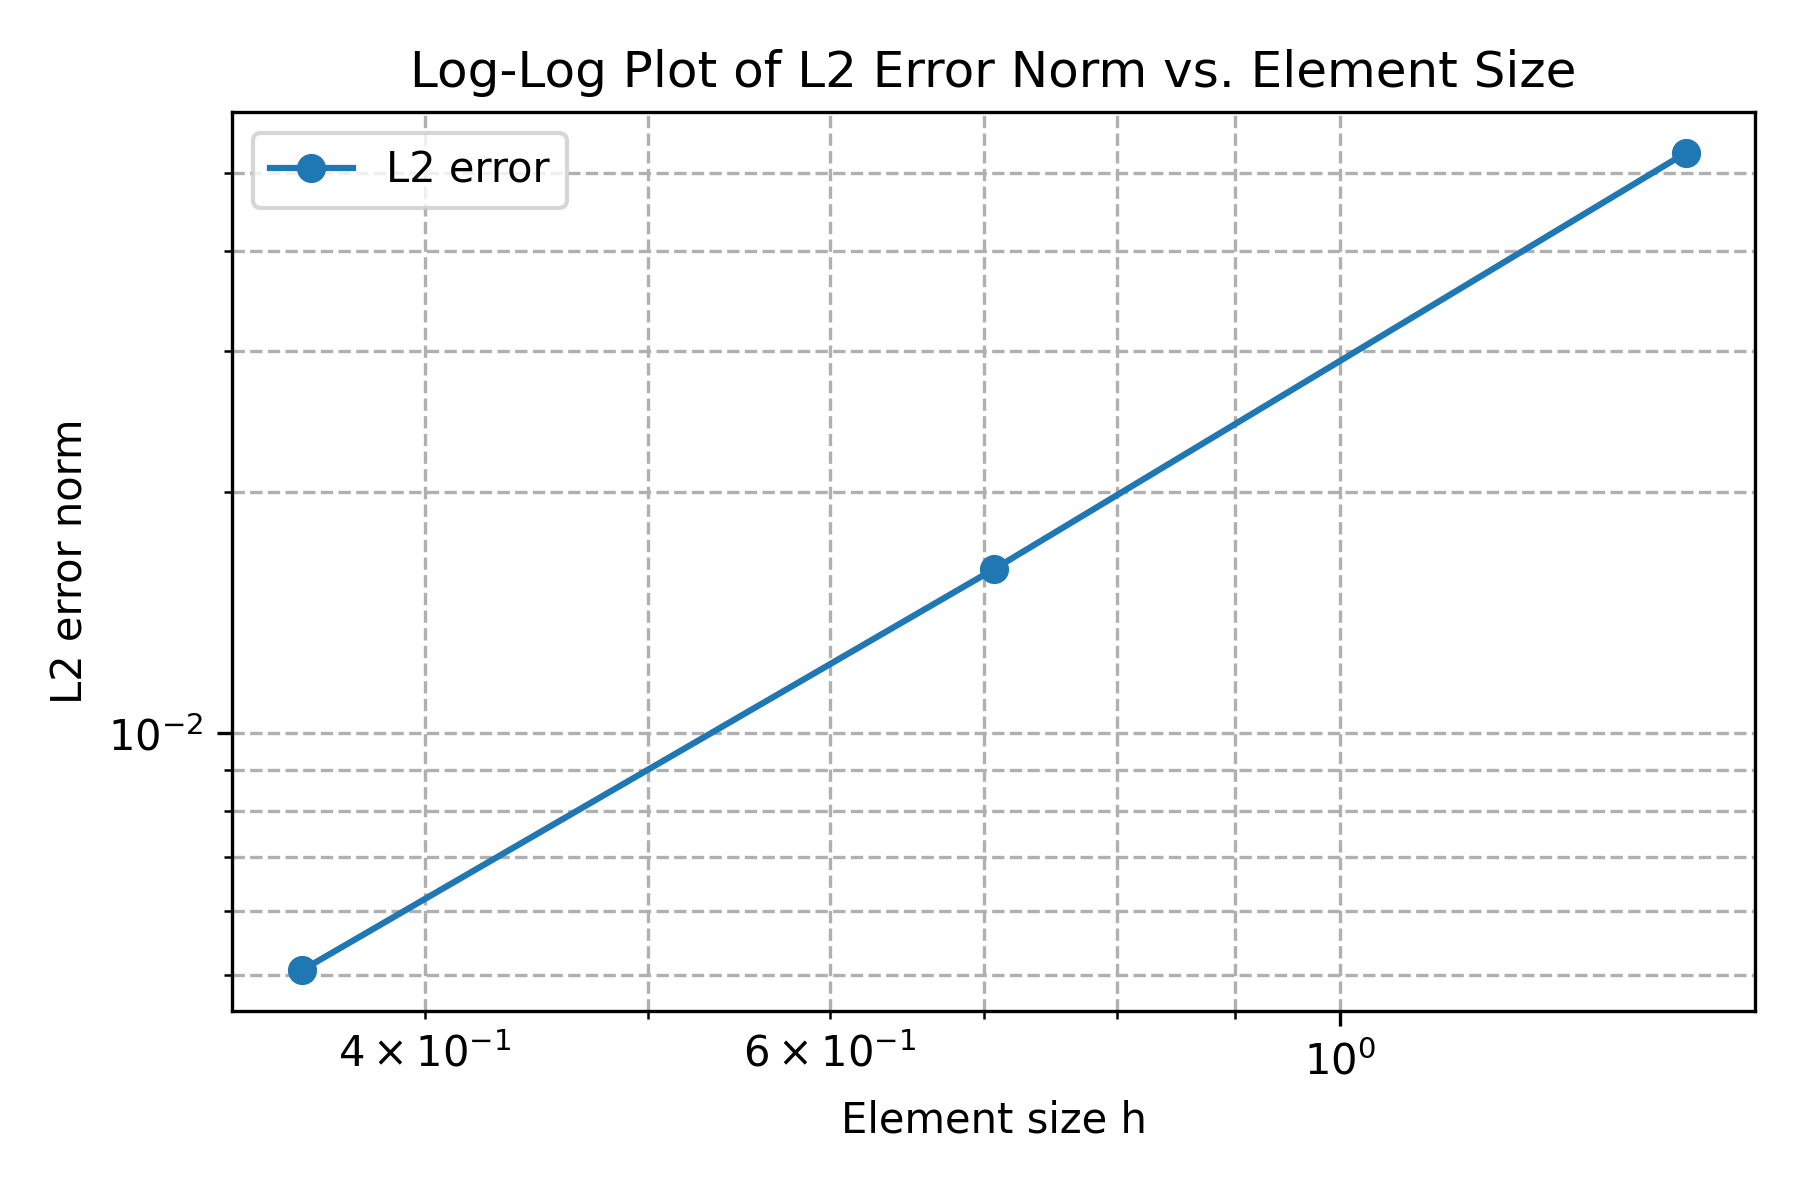
\includegraphics[width=0.6\textwidth]{plotL2.png}
    \caption{Convergence plot of $L^2$ error norm against mesh size $h$}
    \label{fig:convergence_plot}
\end{figure}

\chapter{Conclusion}
Based on the original code, compatibility with planar Q4 elements has been added. The implementation has passed patch tests and convergence analysis. Matrix operation routines and a separate result visualization module have also been added, with well-designed interfaces left in place to facilitate the integration of other elements and features in the future.


\appendix

\clearpage  % <--- 强制新起一页


\begin{thebibliography}{1}

\bibitem{1}
Zhang Xiong, 
\textit{Fundamentals of finite element method},  2023.

\bibitem{2}
Li Hao, 
\textit{https://github.com/Kaishouyue/my-stappp}.


\end{thebibliography}




\end{document}





